% !Mode:: "TeX:UTF-8"
\chapter{基于\texorpdfstring{\(^{99m}\)}{99m}Tc-MDP动态骨显像的假体关节感染辅助诊断框架}

上一章介绍了用于分类和检测任务中的人工智能方法,以及它们在医学影像领域中的结合应用。基于上一章的分析,本章主要研究用于辅助诊断假体关节感染的诊断框架。该框架包括预处理算法和基于时序性影像的分类模型DBS-eNet(Dynamic Bone Scintigraphy effective neural Network, 动态骨显像有效神经网络)\cite{nie2023artificial}。首先,预处理算法从动态骨显像中获取有效信息。然后,由DBS-eNet进一步地提取动态骨显像的时序上生理代谢差异性变化特征和其中每张图像中的组织摄取形态特征来实现疾病的自动诊断。在实验中,该框架和目前主流的分类网络、专业的核医学专家进行了对比,结果表明该方法可以有效且准确地辅助诊断假体关节感染,同时具有潜在的临床应用价值。

\section{问题分析}

在面对动态骨显像中的假体关节感染的诊断任务时,必须综合考虑括医生对假体关节感染的诊断流程、动态骨显像的性质和基于深度学习的辅助诊断框架的有效设计。因此,本文需要思考以下几个问题:

(1)\textbf{关节置换手术后动态骨显像的公开数据集的缺乏}。本文作者与上海市第六人民医院核影像科医生收集了许多患者影像数据并进行了清洗,构建了一个由经历过髋关节置换手术或者膝关节置换手术的患者的真实动态骨显像数据集。然而,该数据集存在着数据规模小、数据不平衡的问题,增加了人工智能诊断框架的设计要求与训练难度。

\begin{figure}[h]
    \centering
    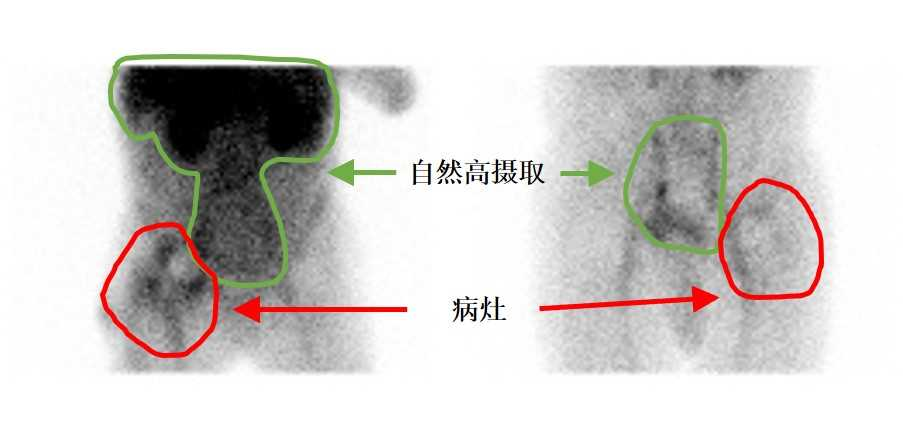
\includegraphics{figures/chap03_hip.jpg}
    \caption{髋关节置换手术后的动态骨显像}
    \label{fig:chap03_hip}
\end{figure}

(2)\textbf{髋关节置换手术后的动态骨显像存在着生理高摄取区域}。在人体的髋部附近存在着膀胱和肾脏这类自然高摄取区域,同时假体关节疼痛区域也会出现高摄取的情况,如图\ref{fig:chap03_hip}所示。这两者的同时出现会导致神经网络在训练过程中产生混淆,无法学习到真实有用的信息,难以关注于病灶区域。

(3)\textbf{动态骨显像本身的影像特点}。动态骨显像包括三种不同条件下采集的影像,分别是在注射后立刻动态扫描(2秒/帧,20帧)用于获取灌注信息的血池相、灌注后动态扫描(1分钟/帧,5帧)可帮助诊断炎症状况或血液供应问题的血流相\cite{schauwecker1992scintigraphic}和在延迟代谢阶段中(示踪剂注射后4小时,1帧)扫描的延迟相。因此,主要存在的问题是需要确定要使用哪些相。

(4)\textbf{动态骨显像具有时间连续性}。动态骨显像中,每张图像拥有组织摄取形态特征,一系列图像之间在时序上存在生理代谢差异性变化特征。因此,如何利用上动态骨显像的时序性特征也是一个需要研究的主要问题之一。

(5)\textbf{神经网络是一个缺乏解释的黑盒}。DBS-eNet是一个端到端的神经网络,可直接通过数据输入到模型之中获得最终结果。这导致医生很难以理解或者分析模型所提取和学习到的相关知识。这不仅缺乏决策过程中的透明性,还没有对模型的决策结果的解释,无法给医生带来可信度以及临床诊断的依据。

在本章研究中,设计了一个基于\(^{99m}\)TC-MDP动态骨显像的框架,用于辅助诊断假体关节感染。该框架针对上述问题一一进行优化改进:

(1)通过使用数据增强方法(镜像、旋转)和损失函数Focal Loss\cite{lin2017focal}上的改进(结合Label smoothing\cite{zhang2021delving}),来解决数据集规模小和数据不平衡的问题。

(2)提出了三种数据预处理算法,分别是标准预处理算法、干扰减少预处理算法和基于感兴趣区域预处理算法,来获取图像序列中有效的信息。其中,标准预处理算法可以用于经历过膝关节置换手术后患者的动态骨显像,同时这三种预处理算法都可以用于经历过髋关节置换手术后患者的动态骨显像。

(3)动态骨显像由血流相、血池相和延迟相组成。由于非感染与感染在延迟相中均可以呈现阳性,而血流相和血池相对于假体关节感染的诊断更具有敏感性。当血池相和血流相呈现阳性表明感染的可能性较大,当血池相和血流相呈现阴性的时候可以排除假体关节感染。由此,本章的研究主要关注于动态骨显像的血流相和血池相。

(4)针对动态骨显像的时序性图像序列特性,提出了一个基于深度学习和多特征的有效神经网络,DBS-eNet。该模型采用了三维深度卷积和卷积长短期记忆网络(Convolution Long Short Term Memory, ConvLSTM)\cite{shi2015convolutional}作为基础构建块,能够提取预处理后的动态骨显像的在影像学特征和时序特征,并且获得最终的预测结果。

(5)为了验证所提出框架的决策结果的有效性和可信度,在专家的建议下,本章引入了用于可视化模型对某一类输入图像的感兴趣区域的Grad-CAM(Gradient-weighted Class Activation Mapping)\cite{selvaraju2017grad}和用于可视化分类模型提取的特征的可区分性的t-SNE(t-distributed Stochastic Neighbor Embedding)\cite{van2008visualizing}。

\begin{figure}
    \centering
    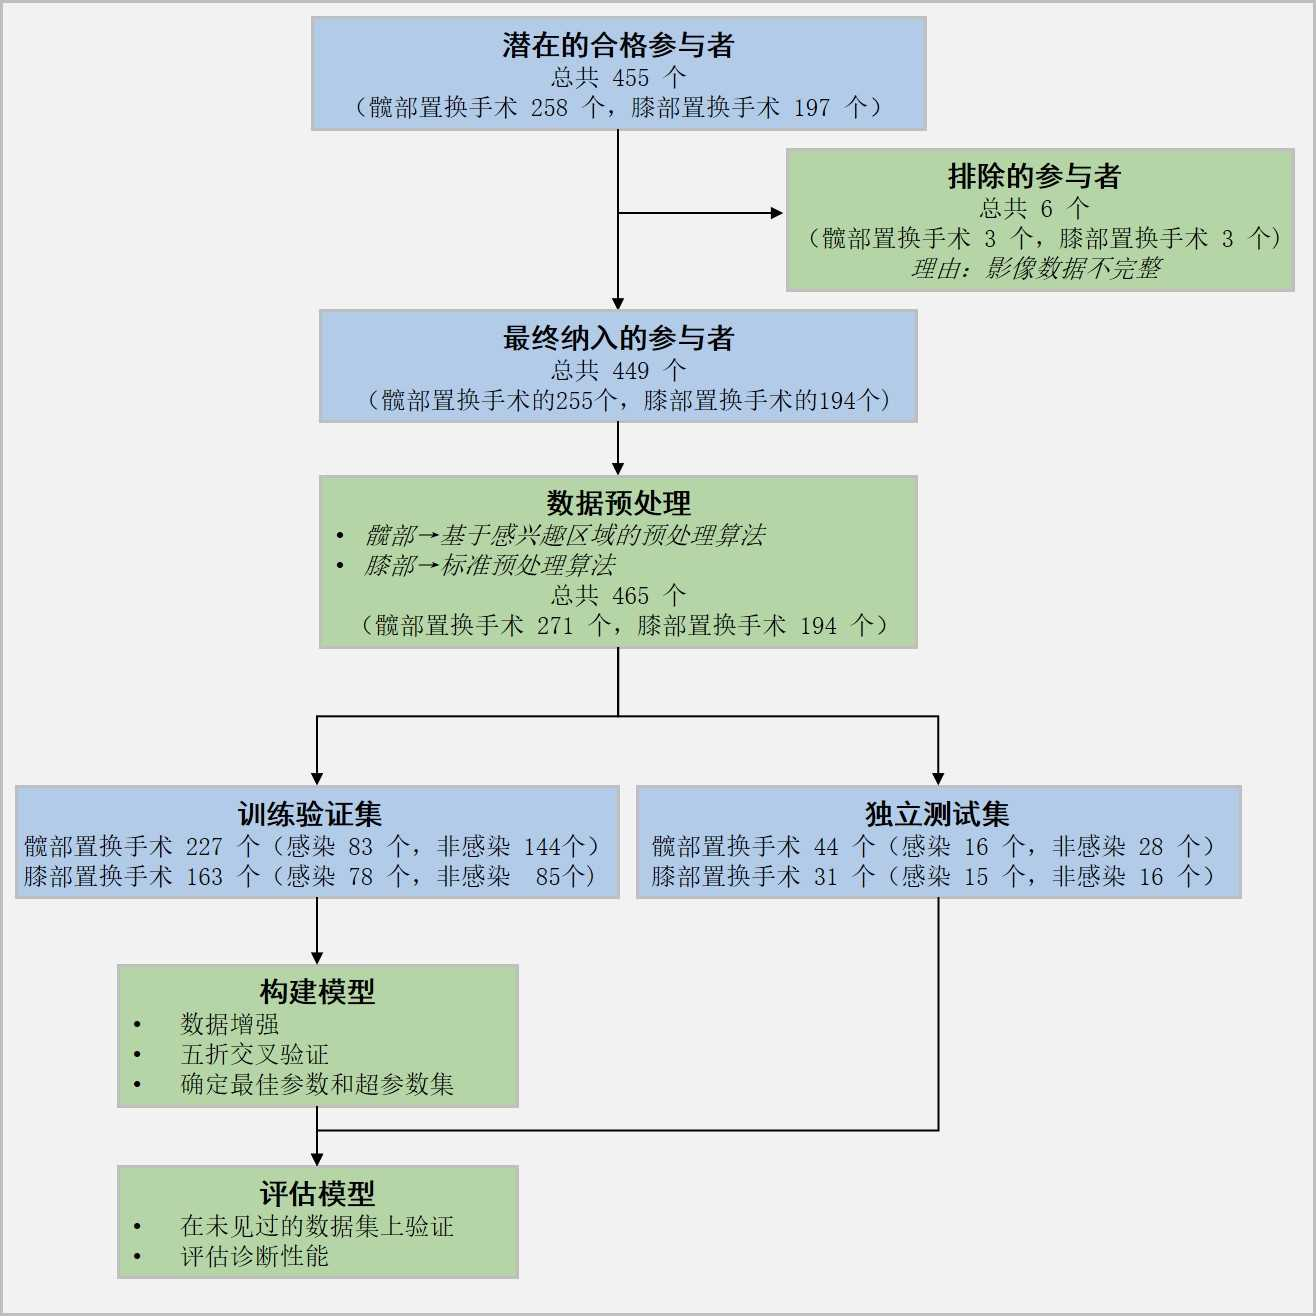
\includegraphics[width=1.0\textwidth]{figures/chap03_workflow.jpg}
    \caption{研究的整体流程:蓝色框表示数据集的信息,绿色框表示对数据集的操作}
    \label{fig:chap03_workflow}
\end{figure}

本章研究的整体流程如图\ref{fig:chap03_workflow}所示。首先,通过最初的数据收集与筛选,最终得到了包含227个髋关节置换手术后的患者数据(感染组与非感染组:83 vs. 144)和163个膝关节置换手术后的患者数据(感染组与非感染组:78 vs. 85)的训练验证集,以及由44个髋关节置换手术后的患者数据(感染组与非感染组:16 vs. 28)和31个膝关节置换手术后的患者数据(感染组与非感染组:15 vs. 16)组成的独立测试集。其次,设计和改良模型结构。通过在训练验证集中五折交叉验证的结果,适应性性地调整模型结构、超参数和训练策略,来获取最终的模型和最佳的超参数。最后,在独立测试集上采用分类任务中的评估指标进一步全面地评估模型的综合性能。

\section{数据预处理}

为了有效地解决动态骨显像数据规模较小、数据集不平衡以及存在自然高摄取区域的问题,本节设计了一个数据预处理流程,如图\ref{fig:chap03_preprocess}所示。通过该流程将动态骨显像转换成有效信息。具体流程如下:

(1)数据清洗与标注:对收集的经历过关节置换手术的患者数据进行清洗,并且进行类别、干扰区域、感兴趣区域的标注;

(2)预处理算法:需要将获取的原生数据转换成可有效区分的数据,去除掉自然高摄取区域的干扰;

(3)数据增强:通过镜像与旋转生成新的数据样本,来增加数据的多样性,以缓解数据集过小的问题。

\begin{figure}
    \centering
    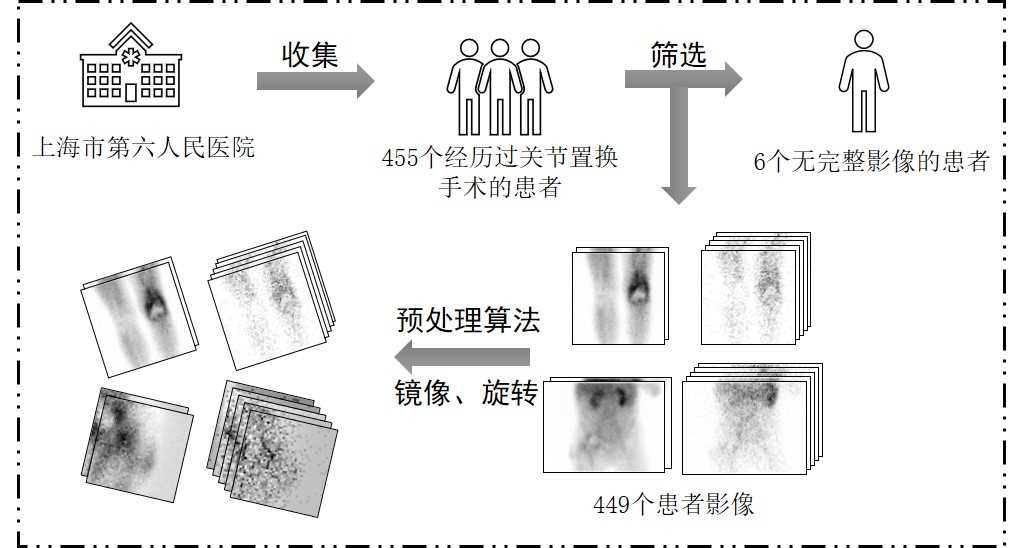
\includegraphics[width=0.8\textwidth]{figures/chap03_preprocess.jpg}
    \caption{针对动态骨显像的数据预处理整体流程示意图}
    \label{fig:chap03_preprocess}
\end{figure}

\subsection{数据清洗与标注}

本章所采集的动态骨显像数据都是以DICOM(Digital Imaging and Communications in Medicine)格式存储。DICOM被广泛用于存储、交换和传输医学图像。作为现代放射成像的核心,DICOM已被医院和医疗软件行业广泛采用,支持各种不同医疗设备获取的影像模态,如超声、CT(Computed tomography)和MRI(Magnetic Resonance Imaging)等\cite{mildenberger2002introduction}。

数据预处理的第一步是对收集到的患者数据进行清洗,如排除掉影像数据不完整、缺乏完整诊断结果的病例。此外,为了保护病人的个人隐私信息,对DICOM格式文件进行脱敏。因此,DICOM格式文件仅仅保留与图像数据相关的信息。在经过上述操作后,本文作者在专业的核医学医生的指导下使用ITK-SNAP软件(v3.8.0,http://www.itksnap.org)对所有的经历过关节置换手术的患者的动态骨显像进行标注,并最终标注结果由专业医学进行了核查。标注根据患者治疗过程中获取的诊断报告为依据,为每一个患者的动态骨显像确定类别信息和位置信息,还为经历过髋关节置换手术的患者的动态骨显像标注了干扰区域和感兴趣区域,如图\ref{fig:chap03_label}所示。

\begin{figure}[t]
    \centering
    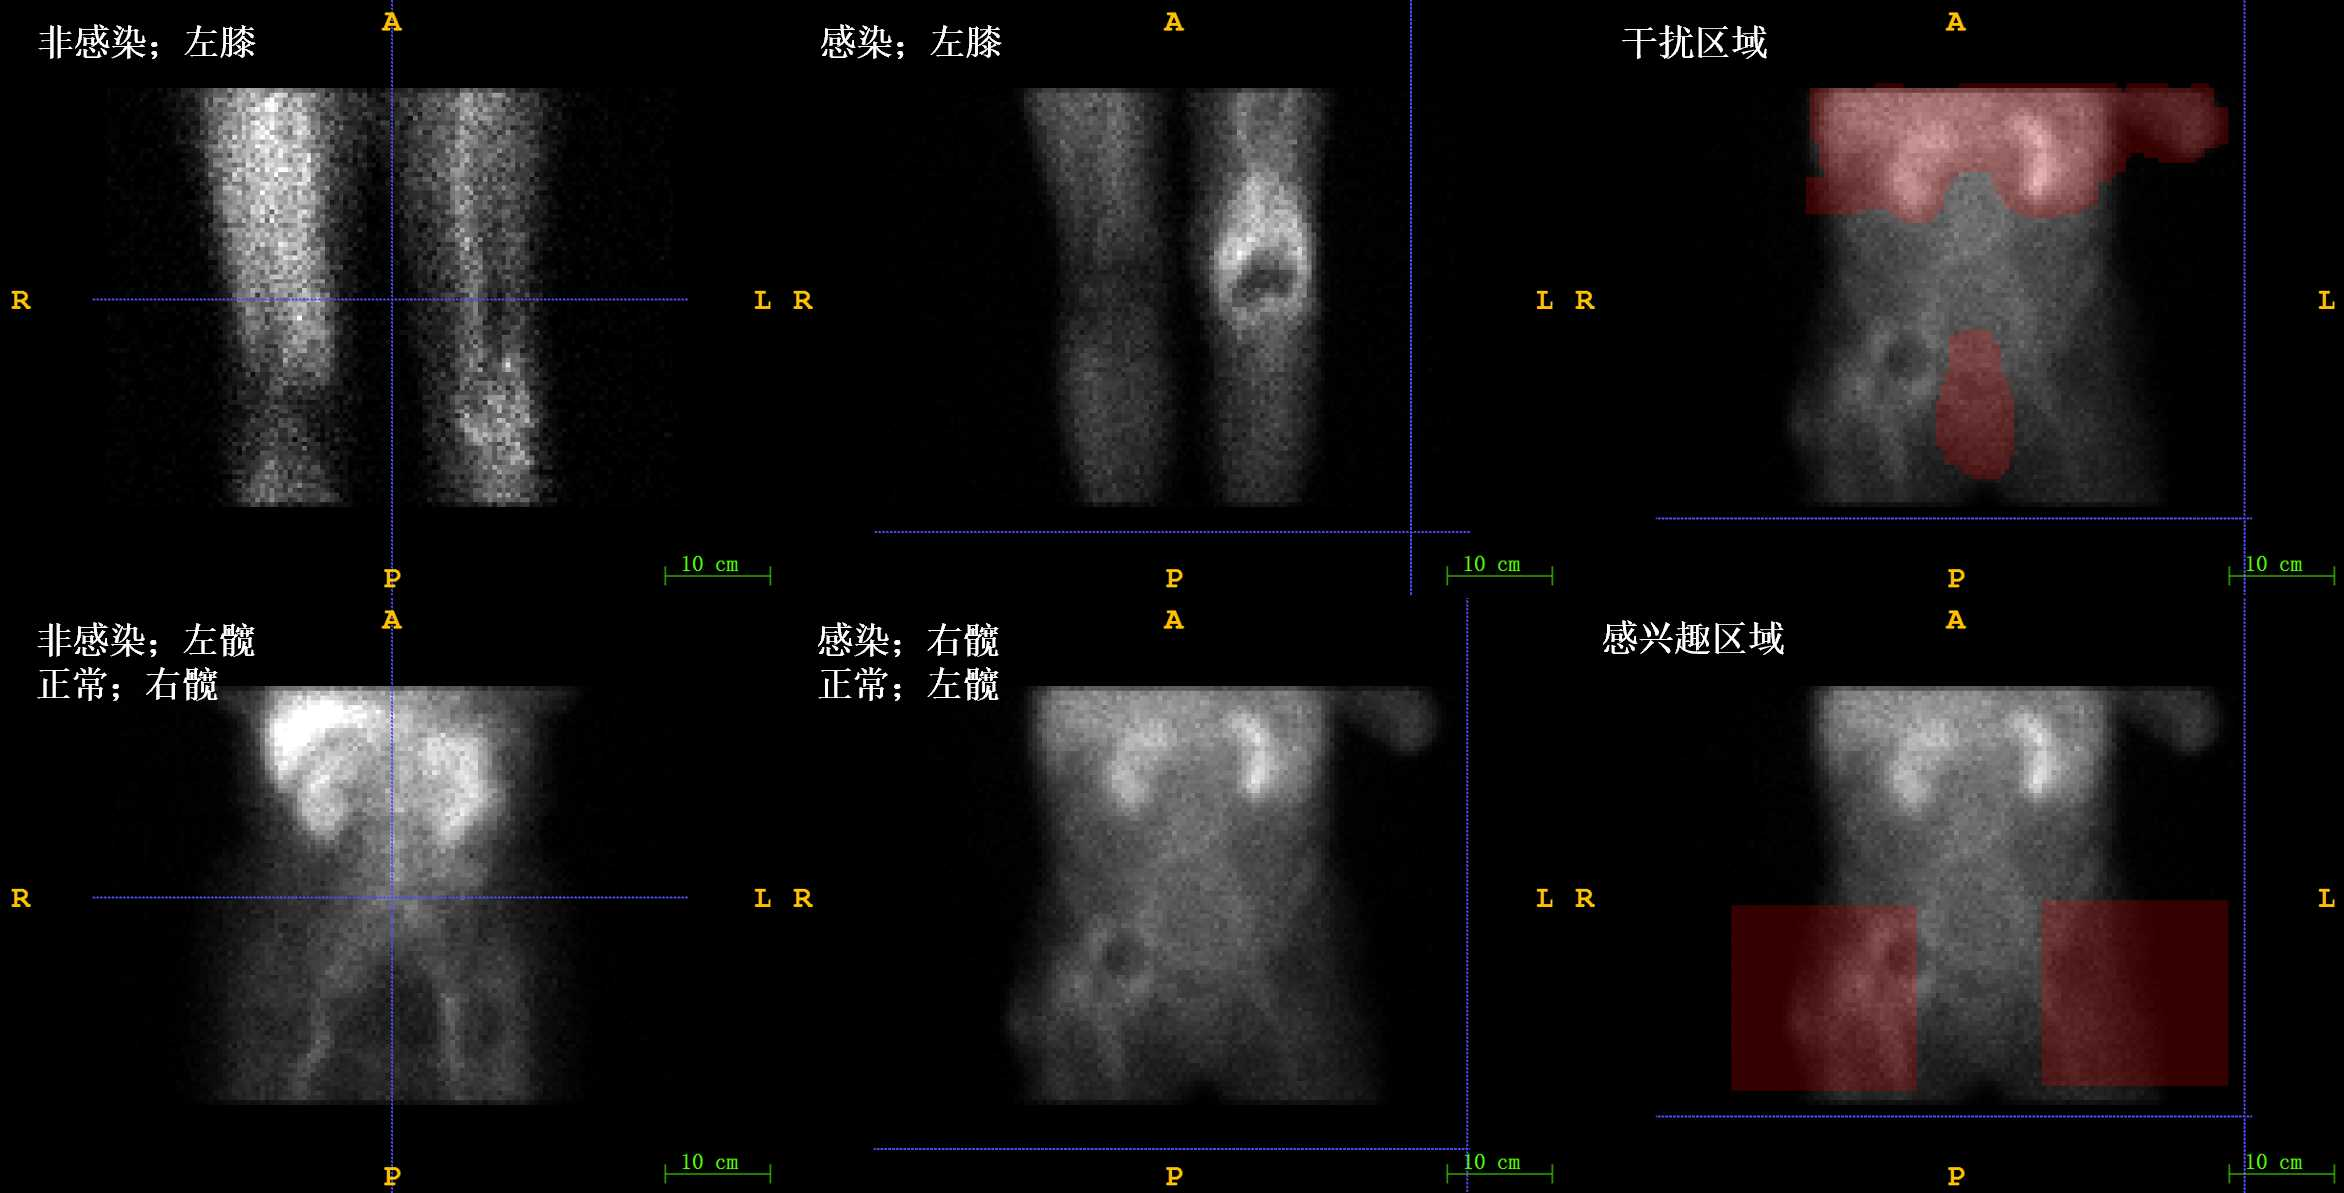
\includegraphics[width=0.8\textwidth]{figures/chap03_label.jpg}
    \caption{动态骨显像的数据标注}
    \label{fig:chap03_label}
\end{figure}

在数据标注完成之后,将对数据进行进一步的整理工作。首先,去除掉数据集中存在的重复的影像数据。其次,将所有的影像数据和标注数据转换为NPZ格式。其中,NPZ格式文件是NumPy\cite{harris2020array}中的一种以二进制的形式存储的格式文件,可用于以未压缩形式的存储多个NumPy数组对象。通过采用NPZ格式文件,将影像数据与它对应的标注数据存放在一个NPZ文件之中。在整理工作完成之后,将最后的数据按照一定的规则放入到相应的服务器位置之中,完成数据预处理首要的准备工作。

\subsection{预处理算法}

由于原生的影像数据在不同个体之间的数值波动范围差异大以及存在自然高摄取区域,会极大地影响分类性能。因此,本节提出了三种预处理算法,将动态骨显像的影像数据转换为有效信息。预处理后得到的影像数据通过可视化后如图\ref{fig:chap03_algorithm}所示。

\begin{figure}
    \centering
    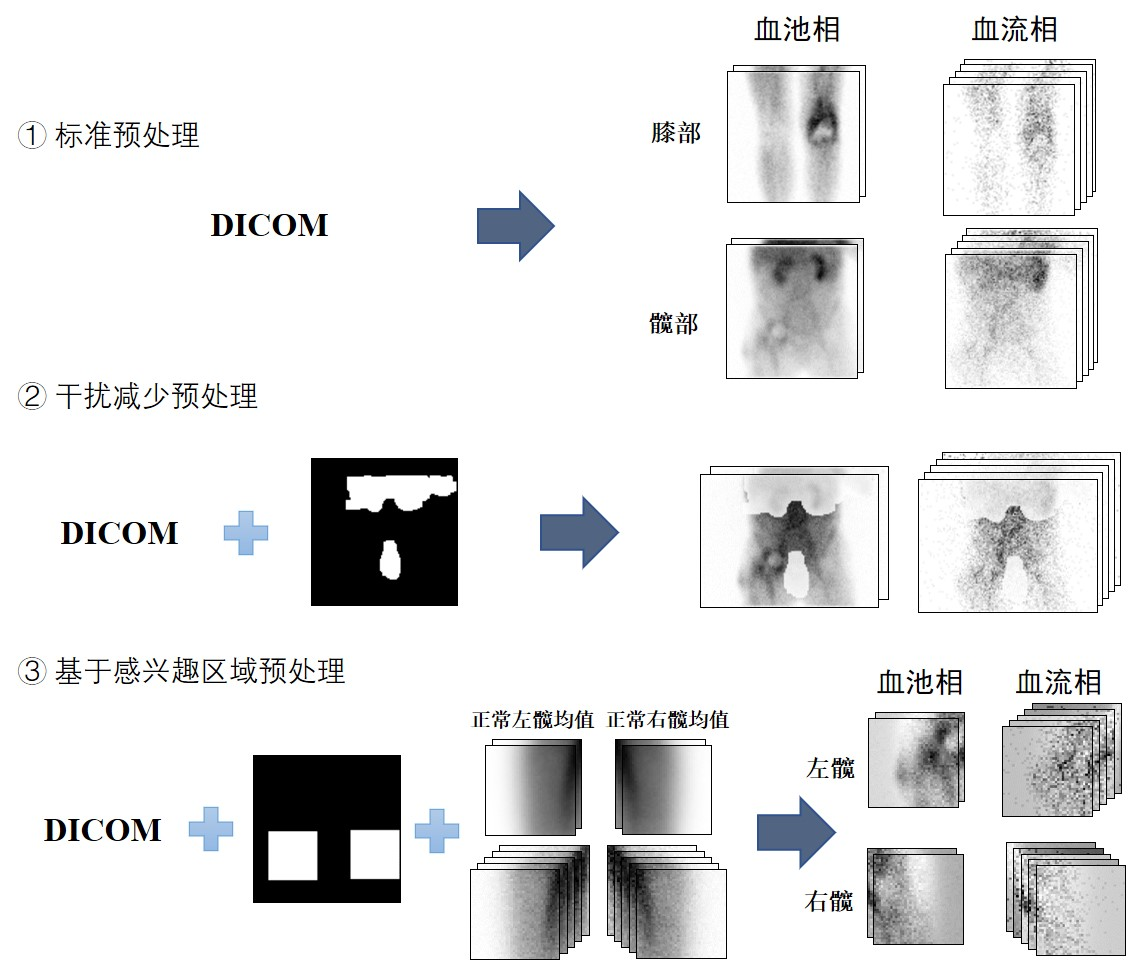
\includegraphics[width=0.9\textwidth]{figures/chap03_algorithm.jpg}
    \caption{三种预处理算法得到的有效信息示意图}
    \label{fig:chap03_algorithm}
\end{figure}

(1)标准预处理

标准预处理的关键步骤就是执行最小最大归一化,通过设定图像数据的下限和上限来调整数据的范围。其基本原理在于病灶区域的上限往往显著高于一般的正常区域,而一般的正常区域的数值范围相对较为固定,因此通过调整图像数据的上限,能够更好地突显出潜在的病灶区域,提高模型对于病变特征的感知能力。标准预处理算法流程如下:

读取\(^{99m}\)Tc-MDP动态骨显像中的血流相\(F\)和血池相\(P\)。其中,血流相\(F\)一共有20张\(128 \times 128\)的二维图像,而血池相\(P\)一共有5张\(128 \times 128\)的二维图像。随后计算出血流相和血池相中的最大值,如公式\ref{eq:chap03_maxmin}:
\begin{equation}
    \begin{aligned}
        F_{max} & = max(max(F_1), max(F_2), \cdots, max(F_{20})) \\
        P_{max} & = max(max(P_1), max(P_2), \cdots, max(P_5))
    \end{aligned}
    \label{eq:chap03_maxmin}
\end{equation}

最后,分别对血流相和血池相数据进行截断和归一化处理,如公式\ref{eq:chap03_standard}所示。
\begin{equation}
    \begin{aligned}
        F_i^{m, n} & =
        \begin{cases}
            1,                           & \text{if \(F_i^{m, n} \geq \alpha F_{max} \)} \\
            0,                           & \text{if \(F_i^{m, n} \leq 0\)}               \\
            F_i^{m, n} / \alpha F_{max}, & \text{otherwise}
        \end{cases} \\
        P_j^{m, n} & =
        \begin{cases}
            1,                           & \text{if \(P_j^{m, n} \geq \alpha P_{max} \)} \\
            0,                           & \text{if \(P_j^{m, n} \leq 0\)}               \\
            P_j^{m, n} / \alpha P_{max}, & \text{otherwise}
        \end{cases}
    \end{aligned}
    \label{eq:chap03_standard}
\end{equation}
其中,\( 1 \leq i \leq 20, 1 \leq j \leq 5, 1 \leq m, n \leq 128 \),\(i, j\)分别表示血流相和血池相中相应序号的图像,\(m, n\)分别表示二维图像中像素的行坐标和列坐标,\(alpha \in [0,1]\)是自定义的超参数,用于调整归一化区间的最大值,默认值为\(0.5\)。

(2)干扰减少预处理

干扰减少预处理在标准预处理的基础上,考虑到了自然高摄取区域这类干扰区域,如肾脏、膀胱,与高摄取的病灶区域具有一定的相似性,减少了神经网络对干扰区域与病灶区域的混淆,用以提升分类模型的性能。对于动态骨显像中的多张二维影像数据,每个值表示在相应的人体位置上吸收药物的大致放射强度。该值越大,表示此处药物吸收得多,代表着此处的生理代谢更加活跃。因此,干扰减少预处理的基本原理是降低自然高摄取区域的放射强度值来减少它的干扰能力。干扰减少预处理算法流程如下:

与标准预处理类似,首先读取动态骨显像中的血流相\(F\)和血池相\(P\)并计算出血流相和血池相中的最大值。然后,如公式\ref{eq:chap03_Interference_reduction}通过干扰区域\(A_{IR}\)来降低自然高摄取区域的放射强度:
\begin{equation}
    \begin{aligned}
        F_i^{m, n} & =
        \begin{cases}
            \alpha_{IR}F_i^{m, n}, & \text{if \((m,n) \in A_{IR}\)} \\
            F_i^{m, n},            & \text{otherwise}
        \end{cases} \\
        P_j^{m, n} & =
        \begin{cases}
            \alpha_{IR}P_j^{m, n}, & \text{if \((m,n) \in A_{IR}\)} \\
            P_j^{m, n},            & \text{otherwise}
        \end{cases}
    \end{aligned}
    \label{eq:chap03_Interference_reduction}
\end{equation}
其中,\(\alpha_{IR} \in [0, 1]\)表示对干扰区域的衰竭程度,默认值为\(0.4\)。

最后,再通过标注预处理中公式\ref{eq:chap03_standard}分别对血流相和血池相数据进行截断和归一化处理。

(3)基于感兴趣区域预处理

基于感兴趣区域预处理流程来源于专业的核医学医生在日常的假体关节感染诊断过程中会对正常髋部与关节置换手术后的髋部进行阅览,然后通过它们之间的差异做出判断。由此,通过基于感兴趣区域处理后将得到差异特征,不同于标准预处理和干扰减少预处理得到的强度特征。基于感兴趣区域预处理的算法流程如下:

首先,根据标注的大小为\(40 \times 40\)的感兴趣区域,从动态骨显像中将该区域裁剪出来。其次,根据类别信息\(c\)和位置信息\(p\),计算正常的左髋和右髋的平均值,如公式\ref{eq:chap03_normalL}和\ref{eq:chap03_normalR}所示。
\begin{equation}
    \begin{aligned}
        FNL_{i}^{m, n} & = mean(\sum_{c_i = \text{正常}, p_i = \text{左} } F_i^{n, m}) \\
        PNL_{i}^{m, n} & = mean(\sum_{c_i = \text{正常}, p_i = \text{左} } P_i^{n, m})
    \end{aligned}
    \label{eq:chap03_normalL}
\end{equation}
\begin{equation}
    \begin{aligned}
        FNR_{i}^{m, n} & = mean(\sum_{c_i = \text{正常}, p_i = \text{右} } F_i^{n, m}) \\
        PNR_{i}^{m, n} & = mean(\sum_{c_i = \text{正常}, p_i = \text{右} } P_i^{n, m})
    \end{aligned}
    \label{eq:chap03_normalR}
\end{equation}
其中,\(i, j, m, n\)与公式\ref{eq:chap03_standard}一致,\(FNL, PNL\)分别表示正常左髋血流相和血池相的平均值,\(FNR, PNR\)分别表示正常右髋血流相和血池相的平均值。

最后,对于其他的经历过关节置换手术的感兴趣区域的血流相和血池相\(FROI, PROI\),将根据公式\ref{eq:chap03_roi}进行计算,获得与正常髋部之间的差异特征。
\begin{equation}
    \begin{aligned}
        FROI_i^{m, n} & =
        \begin{cases}
            FROI_i^{m, n} - FNL_i^{m, n}, & \text{if \(pROI_i = \)左} \\
            FROI_i^{m, n} - FNR_i^{m, n}, & \text{if \(pROI_i = \)右}
        \end{cases} \\
        PROI_i^{m, n} & =
        \begin{cases}
            PROI_i^{m, n} - PNL_i^{m, n}, & \text{if \(pROI_i = \)左} \\
            PROI_i^{m, n} - PNR_i^{m, n}, & \text{if \(pROI_i = \)右}
        \end{cases}
    \end{aligned}
    \label{eq:chap03_roi}
\end{equation}
其中,\(pROI_i\)表示经历过关节置换手术的髋部的位置信息。

\subsection{数据增强}

由于数据集规模较小,为了补充数据集,本节采用了镜像和旋转的方式来对生成新的训练样本。镜像将对整个动态骨显像的血流相和血池相进行相同的水平翻转,同时旋转也是对整个动态骨显像的血流相和血池相从\(-20^{\circ}\)到\(20^{\circ}\)中随机选取一个角度进行旋转。数据增强采用在线策略,即在训练过程中随机地应用在预处理后得到的强度特征或者差异特征。在本章研究中,所有的数据增强方法都将以50\%的概率进行采用。

\section{深度学习方法}

动态骨显像拥有两个具有时序的血流相和血池相,它们展示了一个患者在注射药剂后不同时间点下的状态。由于CNN和ConvLSTM模型在提取特征能力上拥有各自的适用领域,本章提出了结合了CNN和ConvLSTM的DBS-eNet模型。该模型采用了卷积模块对输入的特征进行下采样和图像特征提取,有助于减少模型的计算量和参数量,并且采用了ConvLSTM模块继续丰富图像特征并提取时序特征。卷积和ConvLSTM的组合可以增强对动态骨显像的特征提取能力,为模型提供图像以及时序上的混合特征信息。

\subsection{模型结构}

\begin{figure}[H]
    \centering
    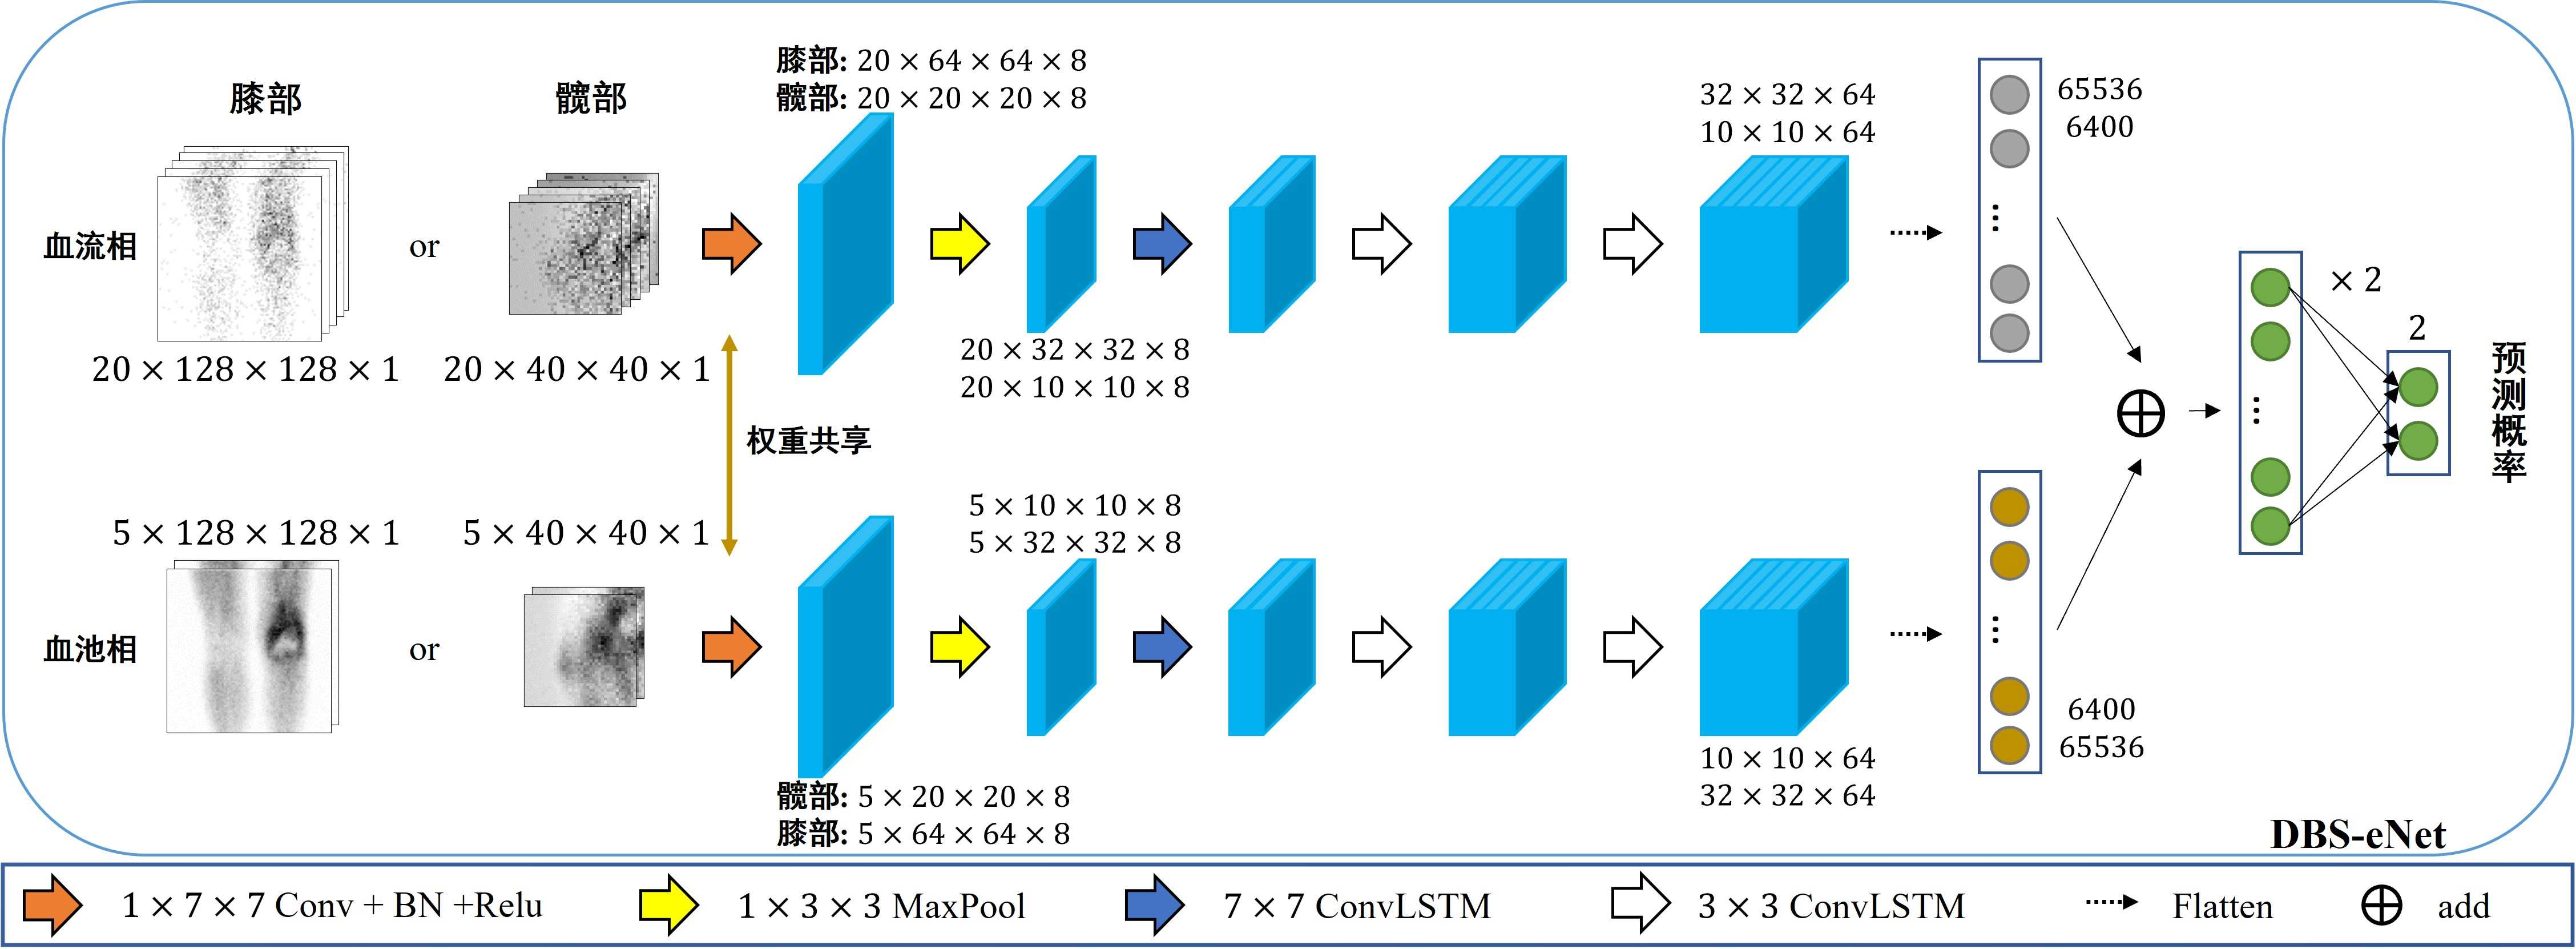
\includegraphics[width=\textwidth]{figures/chap03_framework.jpg}
    \caption{基于深度学习的多特征神经网络模型(DBS-eNet)}
    \label{fig:chap03_framework}
\end{figure}

根据动态骨显像的具有时序性的单通道二维图像,本章针对性地构建了基于深度学习和多特征的有效神经网络DBS-eNet的三个部分。模型结构如图\ref{fig:chap03_framework}所示。

第一部分是一个共享权重且用于提取生理摄取形态特征的\(1 \times 7 \times 7\)的三维卷积层、批归一化层(Batch Normalization)\cite{ioffe2015batch}、校正线性单元(Rectified Linear Unit,ReLU)和用于下采样的最大池化层(Max Pooling)组成。其中,\(1 \times 7 \times 7\)三维卷积层是时序卷积模块,在时序维度上权重的尺寸为1,等价于对每一张图像进行特征提取。又由于血流相和血池相是一个患者在不同时间点下的状态,即在血流相和血池相上病灶区域处于同一位置,因此,时序卷积模块设定为共享权重的形式,去提取血流相和血池相上每一张图像中同一病灶的特征,同时减少参数量;批归一化层用在卷积层之后可以避免数据分布发生变化,用以保留网络各层在训练过程中的学习成果;ReLU激活函数可以有效解决梯度消失的问题并加快收敛速度;最大池化层则可以减少特征的维度的同时提取出特征中更好更强的语义信息。第一部分这样的设计,可以在减少参数量和计算量的同时保持特征的主要语义信息。

第二部分是一个由一层\(7 \times 7\)的ConvLSTM和两层\(3 \times 3\)的ConvLSTM组成。这一设计旨在通过ConvLSTM的结构,在图像处理的过程中更加全面地捕捉和丰富生理形态摄取特征并且在图像序列之中捕获生理代谢差异变化特征。首先,\(7 \times 7\)的ConvLSTM通过大尺寸的卷积核在空间维度上进行卷积,有效地捕捉到图像中的宏观特征。接着,两层\(3 \times 3\)的ConvLSTM通过较小的卷积核在更细致的层次上提取特征,从而使网络能够更灵活地适应各种细节和纹理。最后,ConvLSTM作为长短时记忆网络的一种变体,具有记忆单元和遗忘门等机制,使其能够有效地处理序列数据。通过引入这些时序感知的层,网络不仅可以更好地理解单一图像的内容,还能够在图像序列中建模和捕捉时间上的关联性,从而更全面地分析病灶区域中药剂的摄取形式和程度变化。因此,第二部分的结构在图像特征的丰富性和时序特征的捕获上取得了良好的平衡,为整个模型的性能提供了更强大的表达能力。

第三部分是特征融合层和两层全连接层,融合来自于血流相和血池相中提取的图像特征和时序特征来计算最终诊断结果的概率。首先,特征融合层负责整合不同来源的语义信息,以更全面、准确地反映动态骨显像中图像序列的复杂特征。接着,第一层全连接层引入GELUs(Gaussian error linear units)和Dropout\cite{srivastava2014dropout}。GELUs有助于于引入非线性元素,增强网络对特征的表达能力,同时Dropout则在一定程度上减轻了过拟合的风险,提供了模型的泛化能力。最后,第二层全连接层的输出经过Dropout层的处理,进一步强化了网络对复杂特征的建模能力,并通过Dropout机制降低了过度依赖某些特定特征的风险。第三部分通过这样的设计,有助于确保模型在处理两个不同来源的图像和时序信息的情况下保持稳健性,提供可靠而精准的结果。

\subsection{ConvLSTM}

ConvLSTM是DBS-eNet网络中的核心模块。由于动态骨显像是一个图像序列,重要的不仅是图像特征,还需要捕获整体图像序列之间的时序特征。因此,与简单的卷积神经网络相比,卷积与LSTM相结合的ConvLSTM能够捕获到动态骨显像中的时空特征,更加有效地处理复杂的时序信息,从而使网络在分析动态骨显像时表现得更为出色。

在常见的序列建模模型中,LSTM\cite{memory2010long}作为一种特殊的RNN结构,专门设计来解决传统RNN中存在的梯度消失或梯度爆炸的问题,且已经被证明在建模远程依赖关系方面是稳定而强大的。LSTM的最重要的创新在于记忆单元\(c_t\)和门控机制。记忆单元本质上是一个状态信息的记录器,通过多个门控机制进行更新、清除和输出。每一次有新的输入进来时,如果输入门\(i_t\)被激活,记忆单元里存储的信息将会更新。同样地,如果遗忘门\(f_t\)被激活的话,过去的状态信息\(c_{t-1}\)在这个过程中也将被“遗忘”。最近的记忆单元中的状态信息\(c_t\)是否输出到最终状态\(h_t\),由输出门\(o_t\)控制。通过记忆单元和门控机制来控制信息的流动,可以将梯度留在记忆单元之中,防止梯度太快消失,以更有效地捕捉长期依赖关系。LSTM的关键公式如\ref{eq:chap03_lstm}所示:
\begin{equation}
    \begin{aligned}
        i_t & = \sigma(W_i x_t + U_i h_{t-1} + b_i)                                    \\
        f_t & = \sigma(W_f x_t + U_f h_{t-1} + b_f)                                    \\
        o_t & = \sigma(W_o x_t + U_o h_{t-1} + b_o)                                    \\
        c_t & = f_t \odot c_{t-1} + i_t \odot \text{Tanh}(W_c x_t + U_c h_{t-1} + b_c) \\
        h_t & = o_t \odot \text{Tanh}(c_t)
    \end{aligned}
    \label{eq:chap03_lstm}
\end{equation}
其中,\(\odot\)表示逐元素相乘。多个LSTMs可以堆叠起来形成更加复杂的结构,用以解决更多更复杂的序列建模任务。

尽管LSTM可以解决序列建模任务,但是记忆单元中的状态信息和输出都是一个数值,无法处理更加复杂的序列问题。为了解决这个问题,FC-LSTM\cite{graves2013generating}被提出来,其中它的输入、状态信息和输出均是一维向量。而ConvLSTM在FC-LSTM的基础上进行了扩展,将将输入到状态和状态到状态的转换过程中的全连接结构转换成了卷积结构。为了更好地处理时空数据,ConvLSTM在设计上的显著区别在于输入\(\mathcal{X}_t\)、记忆单元的输出\(\mathcal{H}_t\)和状态信息\(\mathcal{C}_t\)都是二维数据,即空间维度。为了更好地理解输入和状态信息,可以将它们视为一个空间网格。ConvLSTM通过输入和状态信息的局部邻域来确定网格中某个位置的未来状态。这可以很简单地通过卷积操作来实现状态到状态和输入到状态的转变。ConvLSTM的关键公式如\ref{eq:chap03_convlstm}所示:
\begin{equation}
    \begin{aligned}
        i_t           & = \sigma(W_{xi} \ast \mathcal{X}_t + W_{hi} \ast \mathcal{H}_{t-1} + W_{ci} \odot \mathcal{C}_{t-1} + b_i)          \\
        f_t           & = \sigma(W_{xf} \ast \mathcal{X}_t + W_{hf} \ast \mathcal{H}_{t-1} + W_{cf} \odot \mathcal{C}_{t-1} + b_f)          \\
        \mathcal{C}_t & = f_t \odot \mathcal{C}_{t-1} + i_t \odot \text{Tanh}(W_{xc} \ast \mathcal{X}_t + W_{hc} * \mathcal{H}_{t-1} + b_c) \\
        o_t           & = \sigma(W_{xo} \ast \mathcal{X}_t + W_{ho} \ast \mathcal{H}_{t-1} + W_{co} \odot \mathcal{C}_{t} + b_o)            \\
        \mathcal{H}_t & = o_t \odot \text{Tanh}(\mathcal{C}_t)
    \end{aligned}
    \label{eq:chap03_convlstm}
\end{equation}
其中,\(\ast\)表示为卷积计算,\(\odot\)表示逐元素相乘。为了确保状态信息在计算过程中空间大小不变且与输入相同,在进行卷积计算之前需要进行填充(padding)。

\subsection{损失函数}

损失函数用于假体关节感染任务中的作用是评估DBS-eNet网络模型结果的准确程度。由于任务本身收集的髋部数据中存在类别不平衡的情况,不同类别的样本数量差异较大,这可能导致导致模型学习过程中存在一定的偏差。由于感染与非感染的样本分布不均匀,模型可能更容易偏向于在数量中占主导地位的类别,而对于少数类别的样本学习效果相对较弱。为了解决这一问题,本章引入了带有标签平滑(Label smoothing)\cite{zhang2021delving}的\(\alpha\)平衡版的Focal Loss\cite{lin2017focal}用于髋关节置换手术的差异特征信息,用以解决类别不平衡与类别之间的相似性:
\begin{equation}
    \begin{aligned}
        \tilde{y}_{n, c}      & =  \text{Softmax}(x_{n, c}) = \frac{\exp(x_{n, c})}{\sum_{i = 1}^{C}\exp(x_{n, i})}                                                                       \\
        y_{n, c}              & =
        \begin{cases}
            1 - \epsilon         & \text{if \(c = \mathcal{C}\)}    \\
            \frac{\epsilon}{C-1} & \text{if \(c \neq \mathcal{C}\)}
        \end{cases}                                                                                                                \\
        \mathcal{L}_{fl}(x,y) & = -\frac{1}{N}\sum_{n=1}^N \alpha_{n,\mathcal{C}} \cdot (1 - \sum_{c=1}^C \tilde{y}_{n,c}y_{n,c})^{\gamma} \cdot \log\sum_{c=1}^{C}\tilde{y}_{n,c}y_{n,c}
    \end{aligned}
    \label{eq:chap03_THALoss}
\end{equation}
其中,\(x_{n,c}\)是模型的输出结果,表示样本\(n\)对于类别\(c\)的预测值;\(\tilde{y}_{n, c}\)是\(x_{n,c}\)经过Softmax后的预测结果;\(C\)表示类别数量;\(y_{n,c}\)是标签平滑后的真实标签值;\(\epsilon\)是平滑参数;\(\mathcal{C}\)表示正确的类别;\(\alpha_{n,\mathcal{C}}\)表示样本\(n\)对于所属类别\(\mathcal{C}\)的权重因子;\(gamma \geq 0\)表示可调聚焦参数;\(N\)表示批大小。

而对于类别更为平衡的膝关节置换手术的强度特征信息,则采用了加权的交叉熵损失函数:
\begin{equation}
    \begin{aligned}
        y_{n, c}         & =
        \begin{cases}
            1 & \text{if \(c = \mathcal{C}\)}    \\
            0 & \text{if \(c \neq \mathcal{C}\)}
        \end{cases}                                         \\
        \mathcal{L}_{ce} & = -\frac{1}{N}\sum_{n=1}^N\sum_{c=1}^C w_c\log\tilde{y}_{n,c}y_{n,c}
    \end{aligned}
    \label{eq:chap03_TKALoss}
\end{equation}
其中,\(\tilde{y}_{n, c},y_{n,c},C,\mathcal{C},N\)同上式\ref{eq:chap03_THALoss}一致;\(w_c\)表示对于类别\(c\)的权重因子。

\subsection{可视化方法}

为了了解DBS-eNet的决策基础,采用了Grad-CAM和t-SNE。Grad-CAM是一种用于解释深度学习模型预测的可视化技术,特别适用于图像分类任务。其基本原理是在模型通过前向传播预测后计算反向传播的梯度,随后通过对梯度进行全局平均池化得到相应特征图的权重生成类激活图。本章将Grad-CAM应用在框架中的DBS-eNet最后一个ConvLSTM层上来计算类激活图。该类激活图可以显示出动态骨显像中不同区域的重要性。t-SNE是一种降维和可视化高维数据的技术。其核心思想是通过在低维空间中保留原始数据点之间的相似性关系,将高维数据映射到一个更易于理解和可视化的低维空间。本章通过采用保持不同样本之间相对距离的t-SNE方法,将DBS-eNet中提取的最后的特征向量(1024维)降至2维,并将其可视化在二维散点图上来显示出该特征向量的有效性和可区分性。其中,每个点代表在特征空间中的一个感染者或者非感染者的样本。

\section{实验}

\subsection{实验环境}

\begin{table}[htbp]
    \centering
    \caption{实验配置}
    \begin{tabular}{cc}
        \toprule
        环境         & 配置                                     \\
        \midrule
        操作系统     & Linux Ubuntu 20.04.2                     \\
        CPU          & Intel(R) Xeon(R) Gold 5115 CPU @ 2.40GHz \\
        GPU          & NVIDIA Tesla V100, 32GB                  \\
        内存         & 128GB                                    \\
        编程语言     & Python 3.8.17                            \\
        深度学习框架 & Pytorch 1.8.0                            \\
        \bottomrule
    \end{tabular}
    \label{tab:chap03_experimental_config}
\end{table}

本章中的所有实验均在PAI上海大学机器学习平台上进行。该平台是由上海大学计算机学院设计和构建的多加速器异构集群。PAI平台是上海大学首台采用自主开发的基于容器的PAI管理系统的异构计算平台,专注于支持机器学习和深度学习的科研和教学活动。自2018年6月以来,该平台一直提供稳定的计算服务。在硬件方面,该平台包括2个登录/管理节点、1套KNL计算节点、2个FPGA节点、10个双GPU节点、1台配备四个GPU的DGX-station、4个I/O节点,以及一套200T光纤存储阵列,同时配备有1套100G IB高速网络、1套100G OPA高速网络和1套千兆管理网络。这一多样化的硬件配置为各种计算需求提供了灵活的支持。平台的管理软件由上海大学计算机学院自主开发完成,学生们负责相应的软件维护和升级工作。PAI平台不仅面向全校师生提供了丰富的教学资源,还为各类计算任务提供了强大的计算服务。本章的实验的软硬件配置的详细信息如\ref{tab:chap03_experimental_config}所示。

\subsection{数据集}

\begin{table}[htbp]
    \centering
    \caption{动态骨显像的分布情况}
    \begin{tabular}{lcc}
        \toprule
        标签   & 髋关节置换手术 & 膝关节置换手术 \\
        \midrule
        感染   & 99             & 93             \\
        非感染 & 156            & 101            \\
        \bottomrule
    \end{tabular}
    \label{tab:chap03_dataset}
\end{table}

本文作者与上海市第六人民医院核影像科进行合作构建了假体关节感染动态骨显像数据集。该数据集包含髋关节置换手术和膝关节置换手术后的动态骨显像,分类详情见表\ref{tab:chap03_dataset}所示。在数据方面,一共纳入了从2016年1月至2021年6月之间455例具有最终诊断结果的患者,其中258名患者经历了髋关节置换手术,197名患者经历了膝关节置换手术。在查看了所有患者的影像后,其中6例患者由于影像不全被排除。最终纳入并分析了449例患者。所有患者在经历了膝关节置换手术或髋关节置换手术后均出现疼痛或关节功能障碍,且都进行了翻修手术。假体关节感染的最终诊断结果主要基于2021年的EBJIS的定义\cite{mcnally2021ebjis}。本章研究已有的数据集中,最终诊断结果有2个类别标签,感染一共有192例患者的动态骨显像,非感染一共有257例患者的动态骨显像。

\subsection{评估指标}

假体关节感染诊断任务属于分类问题,在评价指标上,本章选用了分类任务中常用的评估指标,如准确率(Accuracy,Acc)、特异率(Specificity,Spec)、敏感率(Sensitivity,Sen)、F1值(F1 Score),阴性预测值(Negative Predictive Value,NPV)、阳性预测值(Positive Predictive Value,PPV)和接收者操作特征曲线下面积(Area Under the receiver operating characteristic Curve,AUC),如式\ref{eq:chap03_metric}所示。
\begin{equation}
    \begin{aligned}
        Acc  & = \frac{TP+TN}{Total}                                         & F1  & = \frac{2 \times PPV \times Sen}{PPV + Sen} \\
        Spec & = \frac{TN}{TN+FP}                                            & Sen & = \frac{TP}{TP+FN}                          \\
        NPV  & = \frac{TN}{TN+FP}                                            & PPV & = \frac{TP}{TP+FP}                          \\
        AUC  & = \frac{\sum_{i \in P} rank_i - \frac{M(1+M)}{2}}{M \times N} &     &
    \end{aligned}
    \label{eq:chap03_metric}
\end{equation}
其中,\(TP,TN,FP,FN\)分别是真阳性、真阴性、假阳性、假阴性样本的数量;\(Total\)表示样本的整体数量;\(P\)表示阳性的类别;\(M,N\)分别是阳性样本和阴性样本的数量;\(rank_i\)是第\(i\)个样本的序号,所有的预测样本根据阳性预测值从小到大进行排序。

准确率表示对假体关节感染预测准确的样本在总样本的占比,但在样本不均衡的情况下,不能够很好地评估模型性能的优劣。特异率表示对实际不患有假体关节感染的患者诊断为未感染的概率。敏感率表示对实际上患有假体关节感染的患者诊断为感染的概率。阳性预测值表示为被诊断为感染的患者实际上患有假体关节感染的概率。阴性预测值表示为被诊断为未感染的患者实际上未患有假体关节感染的概率。F1值是阳性预测值和敏感率的综合评价指标。AUC是敏感性和特异性的综合评价指标。

此外,本章采用了Bootstrap\cite{hesterberg2011bootstrap}来计算这些评估指标的置信区间,并采用麦克内马尔检验(McNemar test)\cite{lachenbruch2014mcnemar}进行统计学分析,来验证DBS-eNet与专业的核医学医生之间的差异性。更进一步地采用了校准曲线(Calibration Curve)和决策曲线分析(Decision Curve Analysis,DCA)\cite{vickers2006decision}来更加全面地评估本章框架的潜在应用价值和有效性。校准曲线(Calibration Curve)可以描绘模型输出的概率与实际观察到的事件发生概率之间的关系,在本章研究中用于评估DBS-eNet预测假体关节感染的概率与实际假体关节感染的概率之间的一致性。决策曲线分析(Decision Curve Analysis,DCA)是一种用于评估预测模型在不同概率阈值下对决策效果的方法。它通常应用于医学领域,特别是在评估临床预测模型的效果,决策曲线分析有助于确定模型在不同概率阈值下相对于其他决策策略的净收益,并为医学决策提供了实用的信息。

\subsection{实验结果}

本章对于构建的动态骨显像数据集先进行上述中的数据预处理后,可以从经历了髋关节置换手术的患者的动态骨显像中获得差异特征(\(25\times40\times40\))以及从经历了膝关节置换手术的患者的动态骨显像中获得强度特征(\(25\times128\times128\)),用于模型训练。对于模型的训练配置,采用了标准的随机梯度下降(Stochastic Gradient Descent,SGD)优化器,初始的学习率设置为0.01,动量(momentum)为0.8,权重衰减(weight decay)为0.0005。批大小(batch size)设置为4,Dropout的比例设置为0.2,以及整个训练周期(epoch)的数量为80。在训练周期的一半和四分之三,学习率将乘以0.1。

为了验证不同预处理算法对于髋关节置换手术数据集的效果,进行了对比实验,如表\ref{tab:chap03_experiment_pre}所示。基于感兴趣区域预处理的效果最佳,优于干扰减少预处理与标准预处理。这是由于基于感兴趣区域预处理,相比较于标准预处理去除掉了自然高摄取区域以外,还使用差异特征替代强度特征,从而避免了在数据集较小的情况下,自然高摄取区域给神经网络带来的偏差干扰。干扰减少预处理则是由于简单但不自然地减弱自然高摄取区域强度的方式,造成了动态骨显像上存在断崖式的强度变化,从而导致了模型的综合性能下降。

\begin{table}[h]
    \centering
    \caption{髋关节置换手术数据集上不同预处理算法下的准确率}
    \begin{tabular}{lcc}
        \toprule
                             & 五折交叉验证 & 独立验证 \\
        \midrule
        标准预处理           & 76.23\%      & 73.21\%  \\
        干扰减少预处理       & 69.32\%      & 68.83\%  \\
        基于感兴趣区域预处理 & 86.33\%      & 86.36\%  \\
        \bottomrule
    \end{tabular}
    \label{tab:chap03_experiment_pre}
\end{table}

\begin{table}[t]
    \centering
    \caption{DBS-eNet在五折交叉验证和独立验证上的综合性能}
    \resizebox{\textwidth}{!}{
        \begin{tabular}{lp{2cm}p{2cm}p{2cm}p{2cm}p{2cm}p{2cm}p{2cm}}
            \toprule
                         & Acc(\%)              & Spec(\%)             & Sen(\%)              & F1                      & PPV(\%)              & NPV(\%)              & AUC                  \\
            \midrule
            \textbf{膝关节置换手术}                                                                                                                                                          \\
            五折交叉验证 & 86.48 (80.98, 91.41) & 83.53 (75.00, 91.25) & 89.67 (82.61, 95.89) & 0.8631 (0.8050, 0.9167) & 84.29 (75.31, 90.81) & 90.83 (82.56, 95.83) & 0.889 (0.825, 0.933) \\
            独立验证     & 87.74 (82.58, 92.90) & 86.25 (78.31, 93.51) & 89.33 (82.19, 95.65) & 0.8772 (0.8182, 0.9290) & 86.60 (77.52, 93.42) & 89.66 (81.92, 95.78) & 0.957 (0.905, 0.973) \\
            \midrule
            \textbf{髋关节置换手术}                                                                                                                                                          \\
            五折交叉验证 & 86.33 (81.50, 90.75) & 92.34 (87.97, 96.38) & 76.03 (67.06, 85.14) & 0.8026 (0.7341, 0.8639) & 86.27 (76.71, 92.86) & 87.12 (81.58, 92.31) & 0.866 (0.809, 0.911) \\
            独立验证     & 86.36 (81.81, 90.91) & 87.86 (82.14, 93.10) & 83.75 (75.31, 91.03) & 0.8178 (0.7464, 0.8784) & 80.25 (70.93, 88.11) & 90.50 (85.50, 94.89) & 0.906 (0.859, 0.946) \\
            \bottomrule
            \multicolumn{8}{l}{\footnotesize 评估指标的值 (95\%置信区间)}
        \end{tabular}
    }
    \label{tab:chap03_ex_DBS-eNet}
\end{table}

本章DBS-eNet的综合性能实验结果如表\ref{tab:chap03_ex_DBS-eNet}所示。在五折交叉验证中,对假体膝关节感染的准确率和AUC值分别为86.48\% (80.98\%, 91.41\%)和0.889 (0.825, 0.933),对假体髋关节感染的准确率分别为86.33\% (81.50\%, 90.75\%)和0.866 (0.809, 0.911)。在独立验证中,对假体膝关节感染的准确率和AUC值分别达到87.74\% (82.58\%, 92.90\%)和0.957 (0.905, 0.973),对假体髋关节感染的准确率分别达到86.36\% (81.81\%, 90.91\%)和0.906 (0.859, 0.946)。这表明了DBS-eNet的综合性能较佳。

为了更好地评估DBS-eNet,实验中采用了五折交叉验证和独立验证的方式。同时,还对比了几个主流的卷积神经网络(VGG\cite{Simonyan2014VeryDC},ResNet\cite{he2016deep},DenseNet\cite{huang2017densely}和ConvNeXt\cite{liu2022convnet})。为了更好地将卷积神经网络应用于预处理后的动态骨显像数据,首先将预处理得到的血池相和血流相数据重采样到\(64 \times 64 \times 64\)。其次,二维卷积神经网络的卷积操作和下采样操作都修改为相应的三维操作。最后,卷积神经网络在卷积部分采用了共享权重,然后提取的特征进行融合并放入全连接层中得到预测结果。

\begin{table}[b]
    \centering
    \caption{DBS-eNet与主流分类网络在五折交叉验证中的平均性能比较}
    \resizebox{\textwidth}{!}{
        \begin{tabular}{lcccccccccccccc}
            \toprule
                        & \multicolumn{7}{l}{膝关节置换手术} & \multicolumn{7}{l}{髋关节置换手术}                                                                                                                                                                                                                               \\
            \cline{2-15}
                        & Acc                                & Spec                               & Sen              & F1              & PPV              & NPV              & AUC            & Acc              & Spec             & Sen              & F1              & PPV              & NPV              & AUC            \\
            \midrule
            VGG11       & 84.05\%                            & 80.00\%                            & 88.67\%          & 0.8407          & 82.76\%          & 90.77\%          & 0.884          & 79.23\%          & 89.58\%          & 60.74\%          & 0.6112          & –                & 81.95\%          & 0.691          \\
            VGG19       & 81.00\%                            & 82.35\%                            & 79.92\%          & 0.7764          & 84.20\%          & 86.13\%          & 0.875          & 81.93\%          & 95.81\%          & 57.79\%          & 0.6988          & \textbf{89.40\%} & 79.84\%          & 0.851          \\
            ResNet18    & 83.37\%                            & \textbf{94.12\%}                   & 71.42\%          & 0.7976          & \textbf{93.04\%} & 79.24\%          & 0.847          & 72.00\%          & 75.17\%          & 66.84\%          & 0.5923          & –                & –                & 0.715          \\
            ResNet50    & 64.36\%                            & 52.94\%                            & 77.08\%          & 0.6763          & 64.07\%          & 73.16\%          & 0.601          & 57.99\%          & 80.00\%          & 20.00\%          & 0.1067          & –                & –                & 0.351          \\
            DenseNet121 & 79.72\%                            & 81.18\%                            & 77.67\%          & 0.7803          & 83.69\%          & 82.68\%          & 0.844          & 79.62\%          & \textbf{95.17\%} & 52.50\%          & 0.5975          & –                & 78.76\%          & 0.791          \\
            ConvNeXt-T  & 52.16\%                            & 100.00\%                           & 0.00\%           & 0.0000          & –                & 52.16\%          & 0.493          & 60.83\%          & 78.62\%          & 29.41\%          & 0.2265          & –                & –                & 0.680          \\
            ConvNeXt-B  & 52.16\%                            & 100.00\%                           & 0.00\%           & 0.0000          & –                & 52.16\%          & 0.432          & 54.94\%          & 57.24\%          & 50.59\%          & 0.3346          & –                & –                & 0.544          \\
            DBS-eNet    & \textbf{86.48\%}                   & 83.53\%                            & \textbf{89.67\%} & \textbf{0.8631} & 84.29\%          & \textbf{90.83\%} & \textbf{0.889} & \textbf{86.33\%} & 92.34\%          & \textbf{76.03\%} & \textbf{0.8026} & 86.27\%          & \textbf{87.12\%} & \textbf{0.866} \\
            \bottomrule
        \end{tabular}
    }
    \label{tab:chap03_DBS-eNet_vs_CNN}
\end{table}

如表\ref{tab:chap03_DBS-eNet_vs_CNN}所示,可以看出DBS-eNet的性能优于其他的卷积神经网络,在膝关节置换手术和髋关节置换手术的五折交叉验证集上都具有最好的准确率、灵敏性、F1值和阴性预测值,以及良好的特异性和阳性预测值。这表明卷积和ConvLSTM的结合相比较于三维卷积更适合于具有时序性的图像序列,能够更有效地捕获动态骨显像中的时空特征信息,有效地提高了动态骨显像的分类性能。

\begin{table}[t]
    \centering
    \caption{DBS-eNet在独立测试集上对经历了髋关节置换手术或髋关节置换手术的患者的综合性能与三名专业核医学医生之间的比较}
    \resizebox{\textwidth}{!}{
        \begin{tabular}{lcccccccccccc}
            \toprule
                     & \multicolumn{6}{l}{膝关节置换手术} & \multicolumn{6}{l}{髋关节置换手术}                                                                                                     \\
            \cline{2-13}
                     & Acc                                & Spec                               & Sen      & F1     & PPV     & NPV      & Acc     & Spec    & Sen     & F1     & PPV     & NPV     \\
            \midrule
            医生1    & 70.97\%                            & 43.75\%                            & 100.00\% & 0.7692 & 62.50\% & 100.00\% & 86.36\% & 89.29\% & 81.25\% & 0.8125 & 81.25\% & 89.29\% \\
            医生2    & 74.19\%                            & 56.25\%                            & 93.33\%  & 0.7778 & 66.67\% & 90.00\%  & 86.36\% & 85.71\% & 87.50\% & 0.8235 & 77.78\% & 92.31\% \\
            医生3    & 74.19\%                            & 50.00\%                            & 100.00\% & 0.7895 & 65.22\% & 100.00\% & 86.36\% & 85.71\% & 87.50\% & 0.8235 & 77.78\% & 92.31\% \\
            DBS-eNet & 87.74\%                            & 86.25\%                            & 89.33\%  & 0.8772 & 86.60\% & 89.66\%  & 86.36\% & 87.86\% & 83.75\% & 0.8178 & 80.25\% & 90.50\% \\
            \bottomrule
        \end{tabular}
    }
    \label{tab:chap03_DBS-eNet_vs_Physician}
\end{table}

此外,本章在独立测试集上将DBS-eNet与3位具有10年以上核医学诊断经验的专家进行比较。为了排除其他因素(例如医生可能接触到某些患者病例),只保留独立测试集中的图像并随机打乱,三位专业核医学专家独立通过各自的临床经验得出诊断结果。比较结果如表\ref{tab:chap03_DBS-eNet_vs_Physician}所示,DBS-eNet在膝关节置换手术的独立测试集上的准确率为87.74\%,高于三位核医学医生的70.97\%、74.19\%、74.19\%。相比之下,DBS-eNet的分类性能与三位核医学医生在髋关节置换手术的独立测试集上能力相当,具有相同的准确率和其他相当的评估指标。三位医师诊断结果与DBS-eNet对经历了膝关节置换手术的患者的预测结果进行比较,\(p\)值分别为0.004、0.008、0.012,均小于0.05,表明该差异有统计学意义。对于经历了髋关节置换手术的患者,三位医师诊断结果与DBS-eNet之间比较的\(p\)值均为1,表明该差异无统计学意义。DBS-eNet的ROC曲线与专家诊断性能如图\ref{fig:chap03_ROC}所示,展示了DBS-eNet与三名专家相当的分类性能。

\begin{figure}[b]
    \centering
    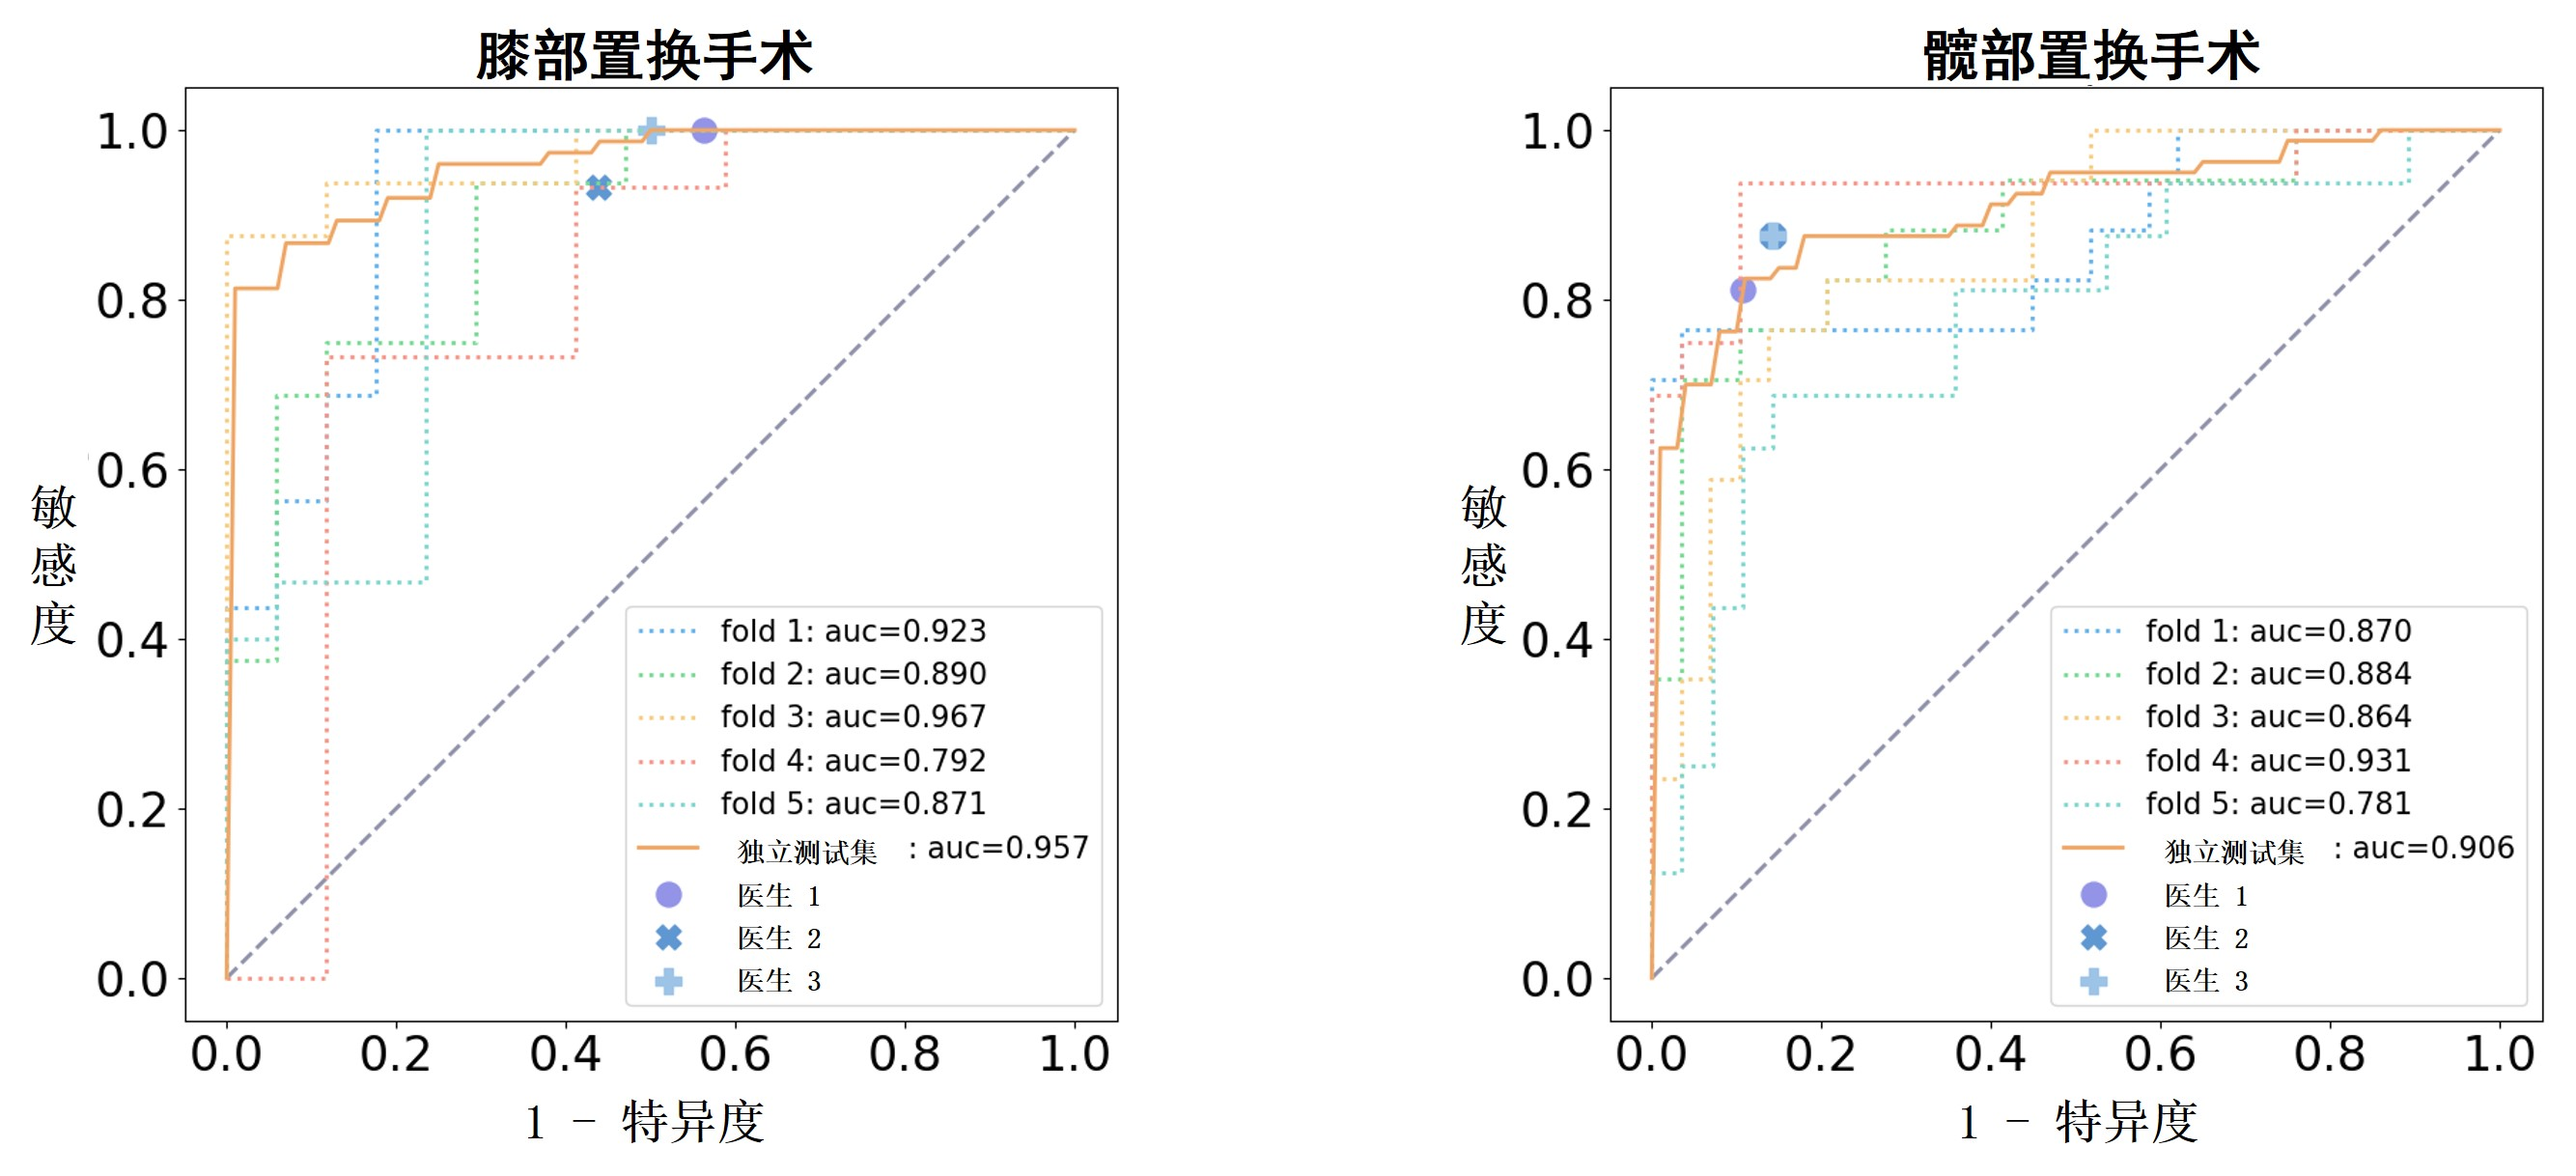
\includegraphics[width=\textwidth]{figures/chap03_ROC.jpg}
    \caption{DBS-eNet在五折交叉验证集和独立测试集上的ROC分析曲线}
    \label{fig:chap03_ROC}
\end{figure}

如图\ref{fig:chap03_CC_DCA}所示,本章提出的框架的校准曲线较为贴近45度对角线,这反映了在膝关节置换手术和髋关节置换手术的动态骨显像数据集上假体关节感染的预测概率与假体关节感染的真实概率具有良好的一致性。此外,本章提出的框架在独立测试集上的决策曲线分析显示,假体关节感染的预测在所有阈值概率下拥有一个较高的净收益,而在五折交叉验证中,存在一到两折在高概率阈值下为负的网络净收益的情况。因此,在大多数情况下,在临床实践中是有价值且有益的。

\begin{figure}[t]
    \centering
    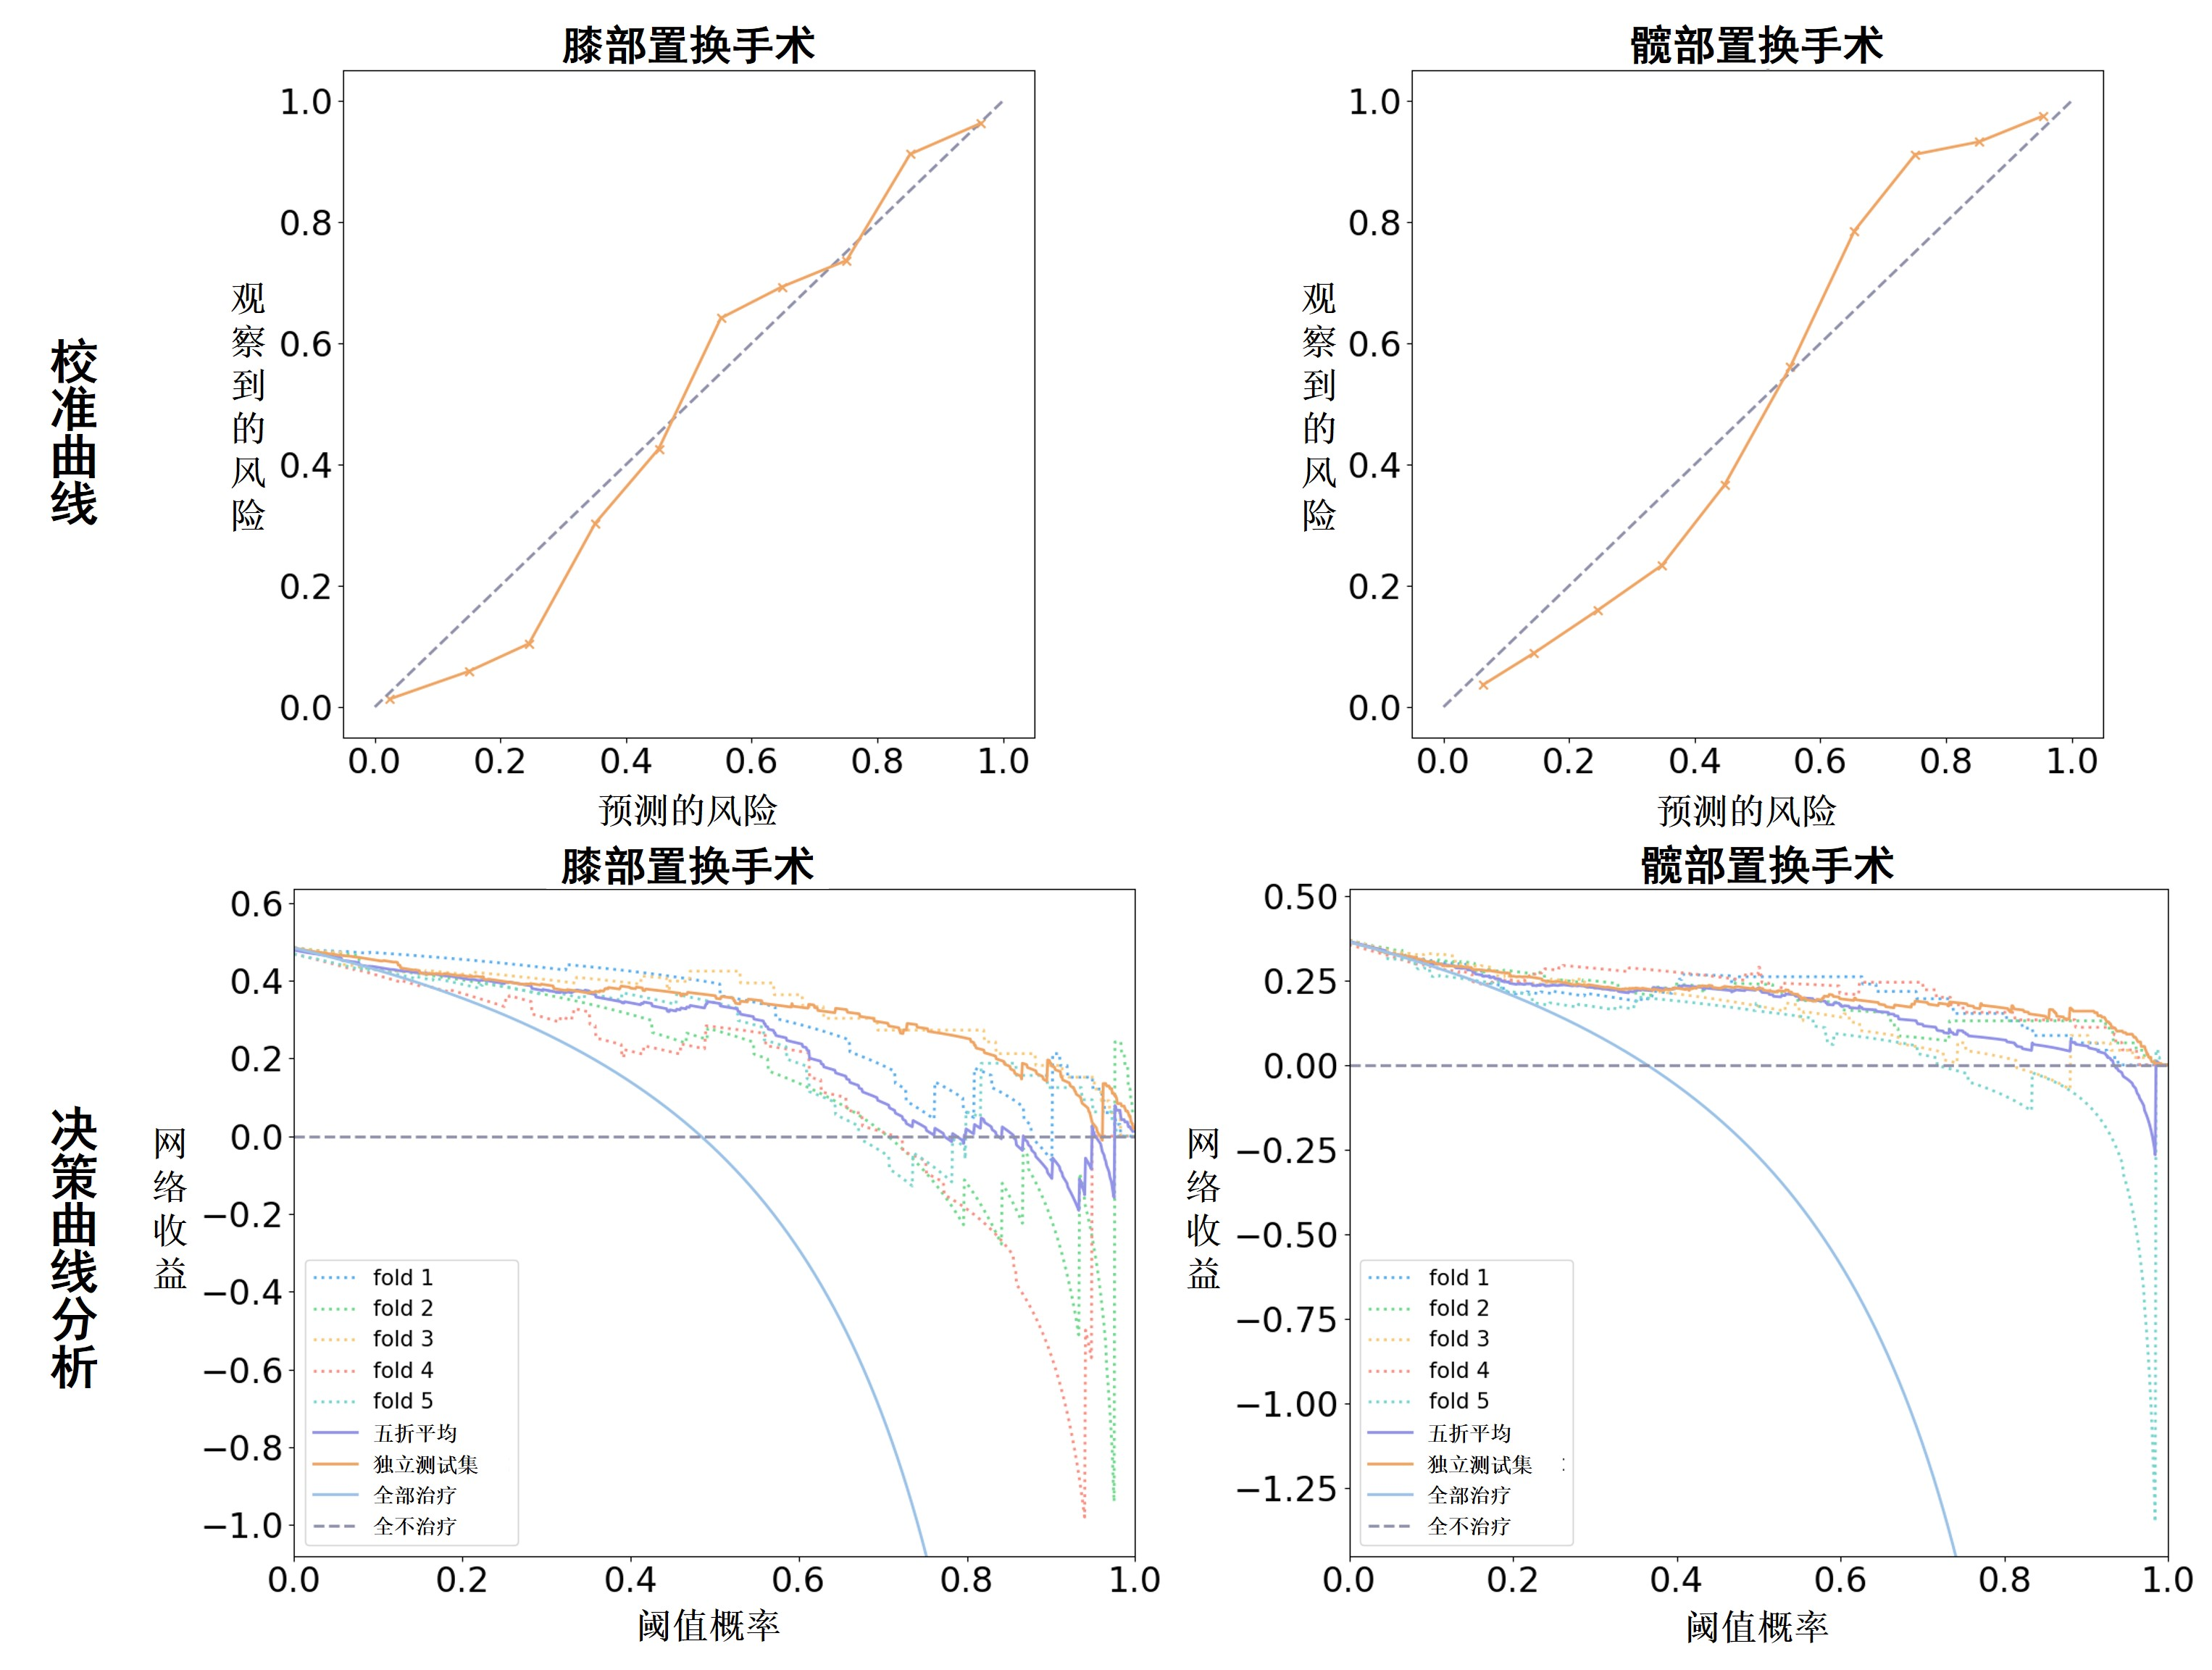
\includegraphics[width=\textwidth]{figures/chap03_CC_DCA.jpg}
    \caption{本文提出的方法在动态骨显像数据集中的校准曲线以及在五折交叉验证集和独立测试集中的决策曲线分析}
    \label{fig:chap03_CC_DCA}
\end{figure}


\subsection{可解释性分析}

动态骨显像与Grad-CAM获得的热力图融合后的图像如图\ref{fig:chap03_Grad-CAM_t-SNE}a所示。动态骨显像中血流相和血池相的病变区域都是重要性最大的区域,这表明DBS-eNet在预测这些影像的最终结果时可以正确聚焦病变区域,也验证了本章提出的方法符合核医学医生在诊断决策中的判断。

在图\ref{fig:chap03_Grad-CAM_t-SNE}b中,t-SNE得到的感染样本和未感染样本的特征点在膝关节置换手术和髋部关节置换手术数据集中都大致地被划分为两簇,体现了DBS-eNet提取的特征本身具有较好的可区分性,表明了该框架的良好性能。通过Grad-CAM和t-SNE方法,可以增加医生对本章提出的方法的可信度。此外,在对经历了关节置换手术的患者进行诊断时,如果医生之间的判定结果一致性较低,通过可视化模型的决策过程以及总结模型学习到的特定模式和影像学特征,这些可以为医生提供额外的意见作为参考,不仅有助于提高疾病诊断的准确率和效率,同时为后续的治疗和预后提供了有力的信息支持。


\begin{figure}
    \centering
    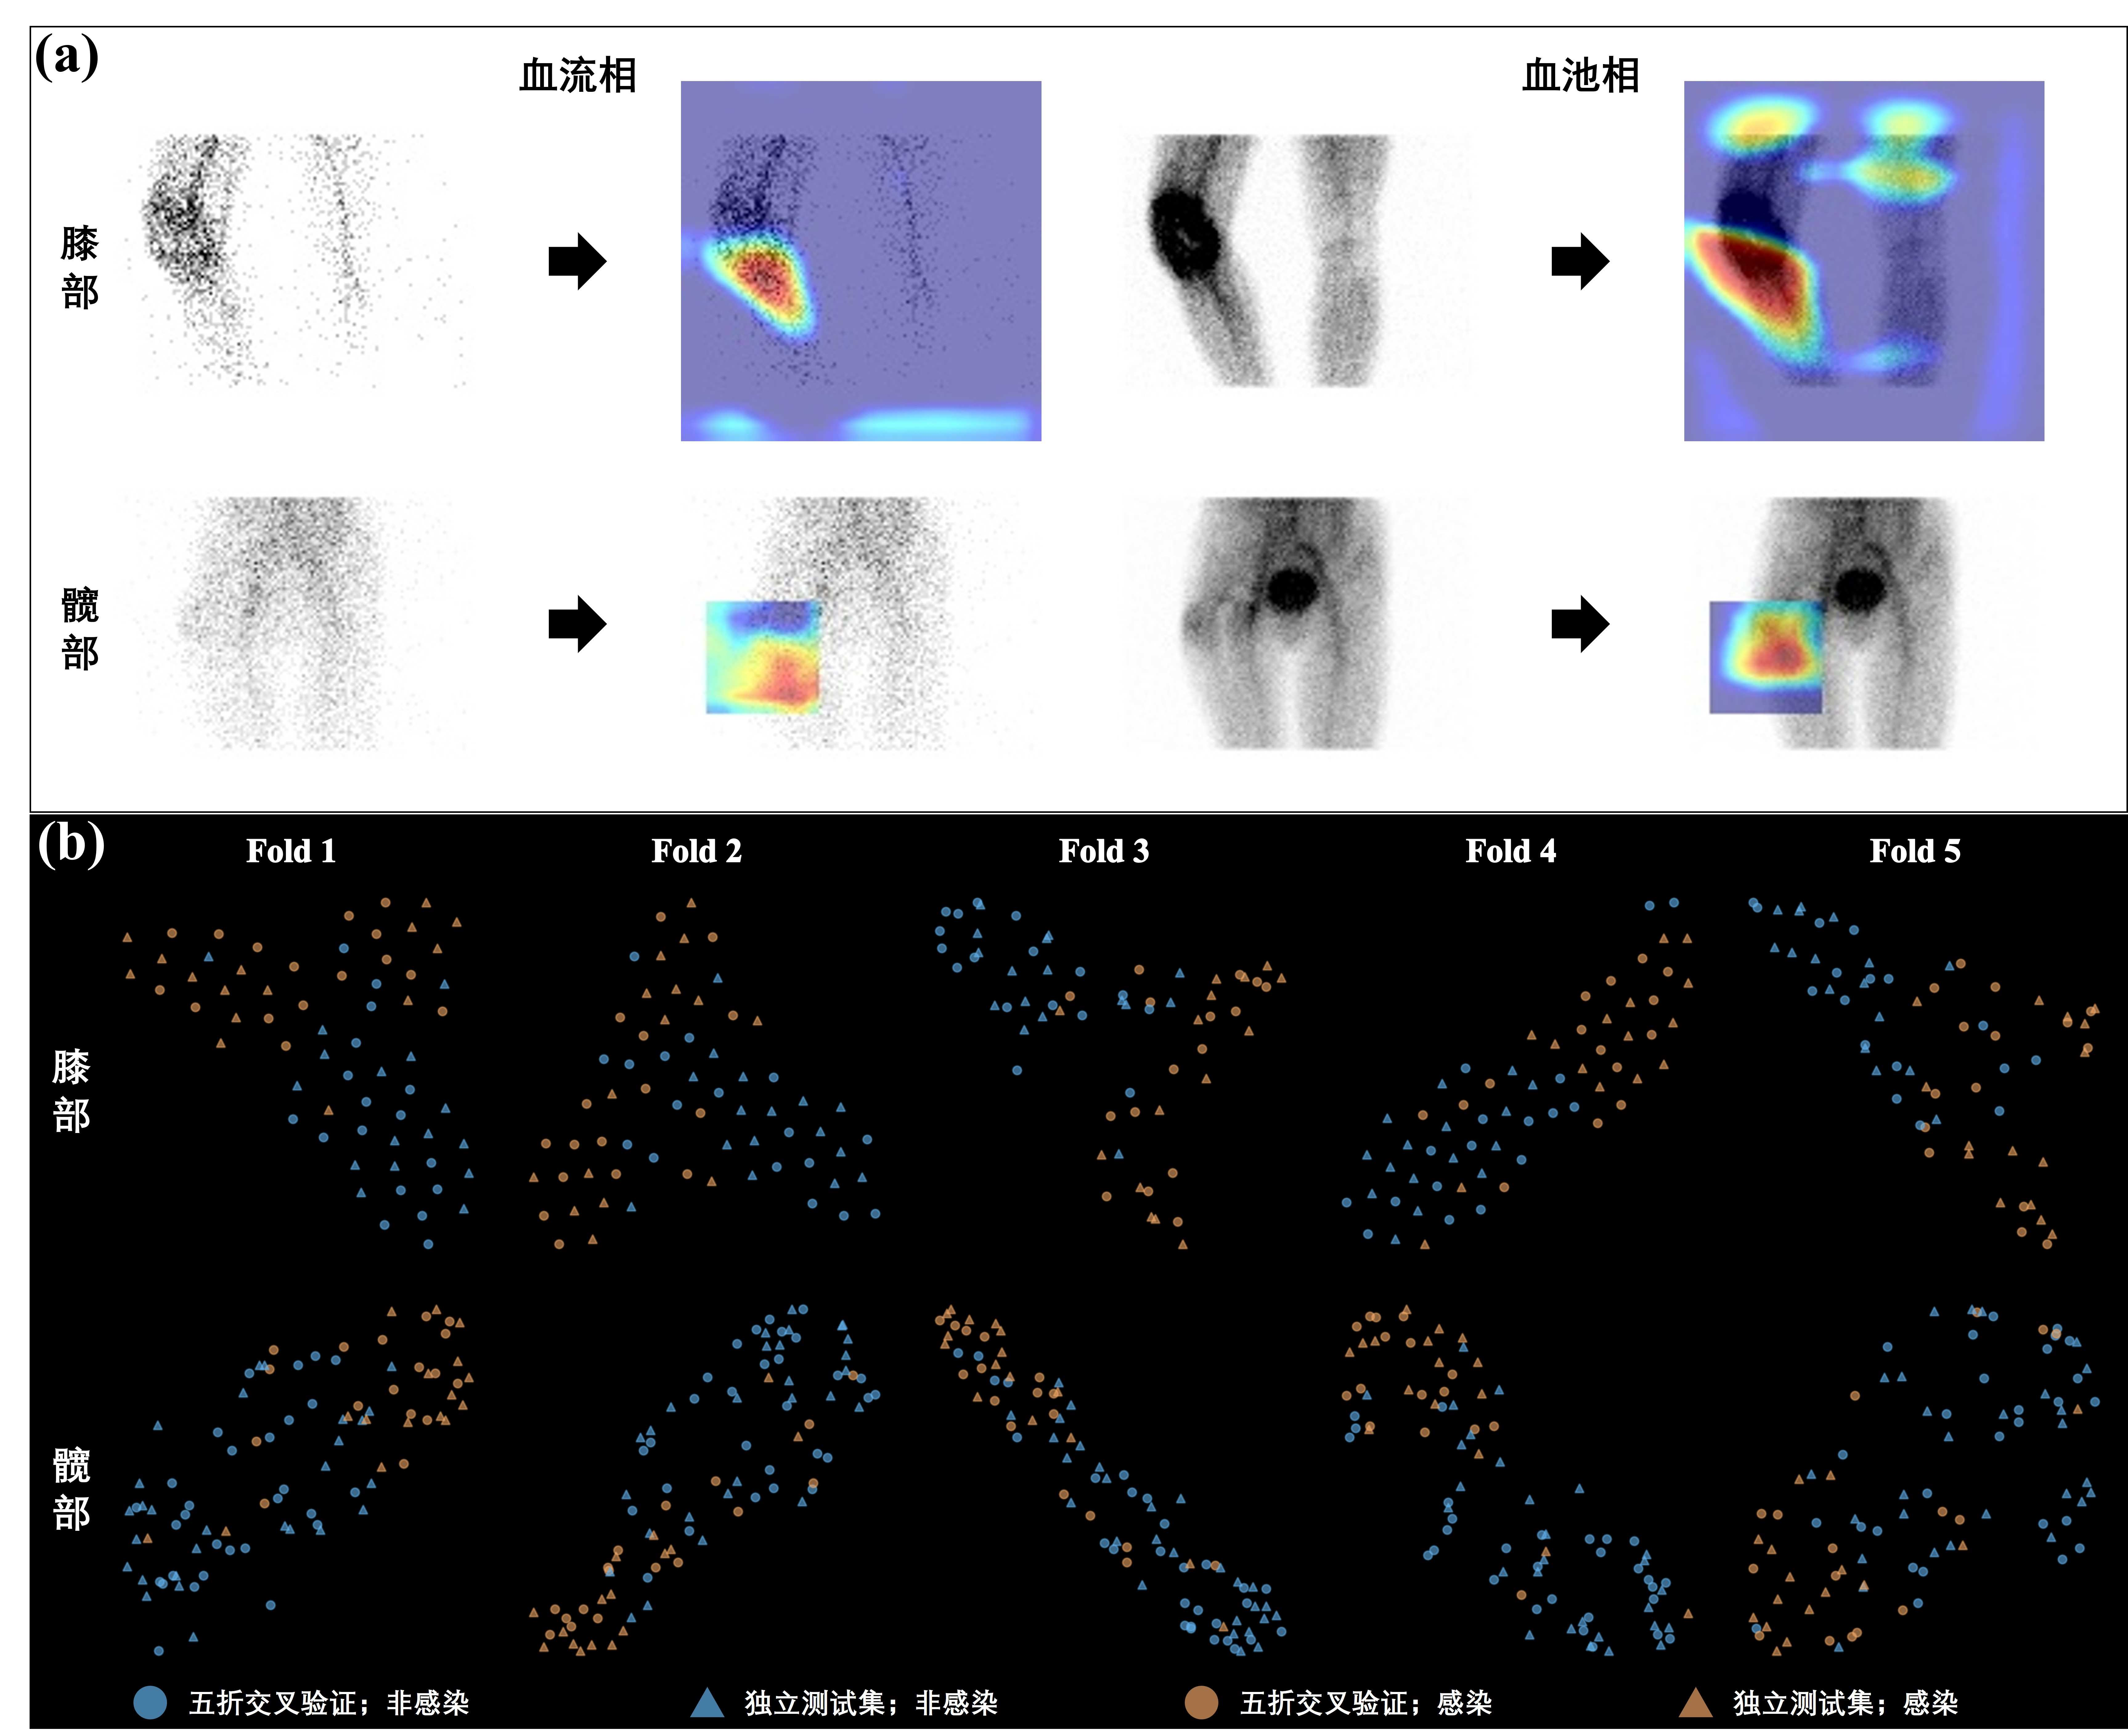
\includegraphics[width=\textwidth]{figures/chap03_Grad-CAM_t-SNE.jpg}
    \caption{\textbf{a} 在DBS-eNet的最后一层ConvLSTM中使用Grad-CAM获得的热图;\textbf{b} DBS-eNet在五折交叉验证集和独立测试集中提取的特征向量进行可视化的t-SNE图}
    \label{fig:chap03_Grad-CAM_t-SNE}
\end{figure}

\section{本章小结}

本章主要提出了一个基于\(^{99m}\)Tc-MDP动态骨显像的假体关节感染诊断框架,由预处理算法和深度学习方法DBS-eNet组成。该框架采用了从膝关节动态骨显像中获取强度特征的标准预处理、从髋关节动态骨显像中获取差异特征的基于感兴趣区域预处理和用来提取每张图像中的生理摄取的形态特征或差异特征和时序上的差异性变化特征的DBS-eNet。在综合性能表现上,该框架在膝关节上达到了86.48\% (80.98\%, 91.41\%)的准确率和0.889 (0.825, 0.933)的AUC,在髋关节上达到了86.33\% (81.50\%, 90.75\%)的准确率和0.866 (0.809, 0.911)的AUC,优于其他卷积神经网络。在与核医学专家的比较中,该框架的性能在诊断假体膝关节感染上优于专家,在诊断髋关节感染上与专家相当。这揭示了人工智能方法在诊断假体关节感染的可行性和诊断框架的有效性。在可解释性分析中,该框架在动态骨显像上关注区域与专家相似,并且提出的特征具有明显的可区分性。这表明它可以有效辅助医生进行诊断决策,提升诊断质量。